\documentclass[11pt,openany]{book}
% ---------------------------------------------------------------------------
% Preamble: typography, math, theorem/exercise machinery, pedagogical boxes.
% ---------------------------------------------------------------------------
% Build with tectonic (XeTeX): native UTF-8, packages fetched on demand.
\usepackage{amsmath,mathtools,bm}         % math BEFORE newpxmath (symbol clashes)
\usepackage{amsthm}
\usepackage{newpxtext,newpxmath}          % Palatino-like text + matching math
\usepackage{microtype}
\usepackage[margin=1.15in]{geometry}
\usepackage{booktabs,tabularx,array,multirow}
\usepackage{enumitem}
\usepackage{graphicx}
\usepackage{xcolor}
\usepackage{tikz}
\usetikzlibrary{positioning,arrows.meta,fit,calc}
\usepackage[most]{tcolorbox}
\usepackage{listings}
\usepackage{caption}
\captionsetup{font=small,labelfont=bf}
\usepackage[colorlinks=true,linkcolor=linkblue,citecolor=linkblue,urlcolor=linkblue]{hyperref}
\usepackage[nameinlink,capitalise]{cleveref}

% ------------------------------------------------------------------- colors
\definecolor{linkblue}{HTML}{2B4C7E}
\definecolor{engbg}{HTML}{EEF3F8}
\definecolor{engframe}{HTML}{2B4C7E}
\definecolor{breakbg}{HTML}{FBEFEA}
\definecolor{breakframe}{HTML}{A84C32}
\definecolor{histbg}{HTML}{F4F1E8}
\definecolor{histframe}{HTML}{8A7B4D}
\definecolor{codebg}{HTML}{F7F7F7}
\definecolor{codeframe}{HTML}{999999}
\definecolor{kwcolor}{HTML}{2B4C7E}
\definecolor{strcolor}{HTML}{7A4A22}
\definecolor{comcolor}{HTML}{6B7B62}

% ------------------------------------------------------------------ listings
\lstdefinestyle{py}{
  language=Python,
  basicstyle=\ttfamily\footnotesize,
  keywordstyle=\color{kwcolor}\bfseries,
  stringstyle=\color{strcolor},
  commentstyle=\color{comcolor}\itshape,
  showstringspaces=false,
  columns=fullflexible,
  keepspaces=true,
  breaklines=true,
  frame=single,
  rulecolor=\color{codeframe},
  backgroundcolor=\color{codebg},
  framesep=4pt,
  xleftmargin=6pt, xrightmargin=6pt,
  aboveskip=8pt, belowskip=8pt,
}
\lstset{style=py}

% ------------------------------------------------------------------ theorems
\theoremstyle{plain}
\newtheorem{theorem}{Theorem}[chapter]
\newtheorem{proposition}[theorem]{Proposition}
\newtheorem{lemma}[theorem]{Lemma}
\newtheorem{corollary}[theorem]{Corollary}
\theoremstyle{definition}
\newtheorem{definition}[theorem]{Definition}
\newtheorem{example}[theorem]{Example}
\newtheorem{exercise}{Exercise}[chapter]
\theoremstyle{remark}
\newtheorem{remark}[theorem]{Remark}

% --------------------------------------------------------- pedagogical boxes
% Engineering consequence: where a piece of theory forces a code decision.
\newtcolorbox{engineering}[1][]{%
  enhanced, breakable, colback=engbg, colframe=engframe,
  boxrule=0.6pt, arc=1.5pt, left=6pt, right=6pt, top=4pt, bottom=4pt,
  title={Engineering consequence\ifblank{#1}{}{ --- #1}},
  fonttitle=\bfseries\small, coltitle=white}

% What breaks: the concrete failure that occurs if the lesson is skipped.
\newtcolorbox{whatbreaks}[1][]{%
  enhanced, breakable, colback=breakbg, colframe=breakframe,
  boxrule=0.6pt, arc=1.5pt, left=6pt, right=6pt, top=4pt, bottom=4pt,
  title={What breaks without this\ifblank{#1}{}{ --- #1}},
  fonttitle=\bfseries\small, coltitle=white}

% Origins: literature and history context.
\newtcolorbox{origins}[1][]{%
  enhanced, breakable, colback=histbg, colframe=histframe,
  boxrule=0.6pt, arc=1.5pt, left=6pt, right=6pt, top=4pt, bottom=4pt,
  title={Origins\ifblank{#1}{}{ --- #1}},
  fonttitle=\bfseries\small, coltitle=white}

% Code walkthrough: annotated excerpts from the real package.
\newtcolorbox{codewalk}[1][]{%
  enhanced, breakable, colback=white, colframe=codeframe,
  boxrule=0.6pt, arc=1.5pt, left=6pt, right=6pt, top=4pt, bottom=4pt,
  title={Code walkthrough\ifblank{#1}{}{ --- \texttt{#1}}},
  fonttitle=\bfseries\small, coltitle=white}

% ------------------------------------------------------------------- macros
\newcommand{\E}{\mathbb{E}}
\newcommand{\Prob}{\mathbb{P}}
\newcommand{\Var}{\operatorname{Var}}
\newcommand{\Cov}{\operatorname{Cov}}
\newcommand{\Corr}{\operatorname{Corr}}
\newcommand{\R}{\mathbb{R}}
\newcommand{\gauss}{\mathcal{N}}
\newcommand{\ind}[1]{\mathbf{1}\{#1\}}
\newcommand{\LSE}{\operatorname{LSE}}
\DeclareMathOperator*{\argmax}{arg\,max}
\DeclareMathOperator*{\argmin}{arg\,min}
\newcommand{\vx}{\bm{x}}
\newcommand{\vy}{\bm{y}}
\newcommand{\vz}{\bm{z}}
\newcommand{\vh}{\bm{h}}
\newcommand{\vpi}{\bm{\pi}}
\newcommand{\IC}{\mathrm{IC}}
\newcommand{\ICbar}{\overline{\mathrm{IC}}}
\newcommand{\ICIR}{\mathrm{ICIR}}
\newcommand{\NLL}{\mathrm{NLL}}
\newcommand{\code}[1]{\texttt{#1}}

% Exercise list at chapter end
\newcommand{\exercisehead}{\section*{Exercises}\addcontentsline{toc}{section}{Exercises}}


\title{\Huge Regime-Conditional Mixture-of-Experts\\[6pt]
       \Large Theory and Engineering of a Quant Research System\\[18pt]
       \normalsize A personal textbook, written against the \code{nec\_baseline} codebase}
\author{Tom Kores Lesjak\\ \small with Claude (Anthropic)}
\date{Draft --- Part I \\ \today}

\begin{document}
\frontmatter
\maketitle

\chapter*{Preface}
\addcontentsline{toc}{chapter}{Preface}

This book exists to answer one question in full: \emph{how do you build a
machine-learning research system for cross-sectional return prediction that
you can actually trust?} Its subject is a single concrete artifact --- the
\code{nec\_baseline} package, a regime-conditional mixture-of-experts written
for a Master's thesis --- but its method is general. Every chapter starts from
a problem you would genuinely face at that stage of the build, develops the
theory needed to solve it, derives the mathematics in full, and only then
shows how the engineering falls out of the theory. Motivation always precedes
mechanism.

Three running principles shape the text.

\emph{First, failure is the curriculum.} The project began as a prototype
that was wrong in eight distinct, instructive ways. Chapter~\ref{ch:autopsy}
performs the autopsy; every later chapter repairs a named defect. When you
meet the mixture negative log-likelihood in Part~II, you will already know
exactly which silent failure it exists to prevent.

\emph{Second, everything is derived.} The reader is assumed to know
probability, linear algebra and basic machine learning at a Master's level,
and nothing else is taken on faith: the EM algorithm's monotonicity, the gate
gradient $\pi - r$, the forward filter, the deflated Sharpe ratio --- all are
derived from first principles, because in this field a formula you cannot
derive is a formula you cannot debug.

\emph{Third, honesty over impressiveness.} Quantitative research has a
structural bias toward self-deception: a leak or a lucky seed always
\emph{improves} a backtest, so errors are asymmetrically rewarded. The
engineering discipline in this book --- data contracts, planted-truth tests,
purged evaluation, trial registries, pre-registration --- is not software
aesthetics. It is epistemology made executable. Where the project has a known
limitation, the book says so plainly, because the defensible posture is the
entire point.

\paragraph{How to read.} The parts are designed to be read in order on a
first pass. Each chapter ends with exercises --- a mix of pen-and-paper
derivations and hands-on tasks against the real codebase --- with solutions in
Appendix~\ref{app:solutions}. Boxes punctuate the text:
\emph{Engineering consequence} (where theory forces a code decision),
\emph{What breaks without this} (the concrete failure that occurs if the
lesson is skipped), \emph{Origins} (where the idea comes from in the
literature), and \emph{Code walkthrough} (annotated excerpts from the real
package). The companion reference for day-to-day use of the code is
\code{nec\_baseline/HANDBOOK.md}; this book teaches you to be the person who
could have written it.

\tableofcontents

\mainmatter

% ===================================================================== PART I
\part{The Problem}\label{part:problem}

\chapter{Predicting the Cross-Section}\label{ch:cross}

\begin{quote}\small\itshape
Before any model, understand the substrate. Cross-sectional return prediction
is not a hard instance of a standard machine-learning problem; it is a
different problem wearing the same clothes. This chapter fixes the task,
quantifies exactly how faint the signal is, and identifies the four features
of the environment --- noise, drift, dependence, and asymmetric error rewards
--- that dictate every design decision made in the rest of the book.
\end{quote}

\section{The object of study}\label{sec:object}

\subsection{Panels}

Everything in this book lives on a \emph{panel}: a set of entities (stocks)
observed jointly over time. Let $t = 1, \dots, T$ index trading dates and let
$\mathcal{U}_t$ denote the \emph{universe} at date $t$ --- the set of names we
are willing to trade and able to observe, with $N_t = |\mathcal{U}_t|$. The
universe changes over time as firms list, delist, merge, and enter or leave
an index; Chapter~13 is devoted to why getting $\mathcal{U}_t$ right (and not,
say, using today's universe throughout history) is a first-order correctness
issue rather than a detail.

For each name $i \in \mathcal{U}_t$ we observe features and, later, a
realized outcome:

\begin{definition}[The prediction task]\label{def:task}
At each date $t$, given features $\vx_{i,t}$ for every $i \in \mathcal{U}_t$,
produce scores $s_{i,t} \in \R$. The target is the \emph{forward return} over
a horizon of $h$ days,
\[
  y_{i,t} \;=\; \frac{P_{i,t+h} - P_{i,t}}{P_{i,t}},
\]
where $P_{i,t}$ is the (dividend- and split-adjusted) price. The task is
\emph{cross-sectional}: what is graded at date $t$ is the correspondence
between the ranking of $\{s_{i,t}\}_{i \in \mathcal{U}_t}$ and the ranking of
the realized $\{y_{i,t}\}_{i \in \mathcal{U}_t}$.
\end{definition}

Two structural remarks, both of which will matter enormously.

First, note what the task is \emph{not}. It is not forecasting the market:
whether stocks collectively rise or fall tomorrow contributes nothing to the
grade, because a constant added to every $y_{i,t}$ leaves all rankings
unchanged. The time-series problem (``will the index go up?'') and the
cross-sectional problem (``which names will outperform which?'') are
different problems with different difficulty profiles, and this book is about
the second. This is also an economic choice: a portfolio built to be long the
top-ranked names and short the bottom-ranked ones, in equal dollar amounts,
is approximately immune to the market's direction --- it monetizes exactly
the ranking skill being graded and nothing else. Chapter~16 makes this
construction precise (quantiles, turnover, costs); Chapter~13 goes further
and makes the \emph{target} itself market-neutral by residualizing returns
against a rolling market beta.

Second, the label spans time. The target $y_{i,t}$ is not knowable until date
$t+h$: a ``sample'' dated $t$ quietly reaches $h$ days into the future. This
banal observation has a sharp consequence --- any evaluation split that puts
date $t$ in the training set and any of $t+1, \dots, t+h$ in the test set has
\emph{leaked test-period prices into training labels}. The purging rule of
Chapter~15 (drop the last $h$ training dates before every test block) is
nothing more than this paragraph turned into an inequality, but the
prototype dissected in Chapter~\ref{ch:autopsy} is far from the only system
to have missed it.

\subsection{Two kinds of features}

The package splits features into two tensors, and the split is conceptual,
not cosmetic:

\begin{center}
\small
\begin{tabular}{@{}lll@{}}
\toprule
 & shape & meaning \\
\midrule
$\vx^{\text{seq}}_{i,t}$ & $(T_w, d_{\text{seq}})$ &
  a trailing \emph{window} of $T_w$ days of per-day channels \\
 & & (returns, ranged volatility, volume shocks, \dots) \\
$\vx^{\text{snap}}_{i,t}$ & $(d_{\text{snap}},)$ &
  a \emph{snapshot} of characteristics known at $t$ \\
 & & (momentum, size, short-horizon reversal, \dots) \\
\bottomrule
\end{tabular}
\end{center}

The sequence tensor exists to be summarized by a recurrent encoder into a
\emph{state}: ``what kind of market has name $i$ been living in lately?'' The
snapshot tensor carries the cross-sectional characteristics that actually
differentiate names on a date. Keeping them separate keeps a later question
crisp --- \emph{who gets to see what?} In the architecture of Part~III, the
encoder's summary drives the regime gate, while the experts read the
snapshot; whether the experts should \emph{also} see the encoder state is a
genuine design decision (Decision~A) with arguments on both sides, and it is
decided, documented, and made switchable rather than picked silently.

Every feature carries one non-negotiable invariant:

\begin{definition}[Point-in-time discipline]\label{def:pit}
A feature value $\vx_{i,t}$ may depend only on information available at or
before date $t$. The target $y_{i,t}$ is the \emph{only} forward-looking
quantity in the panel, and it never appears inside a feature tensor.
\end{definition}

Definition~\ref{def:pit} sounds too obvious to state. It is stated because
violating it is the single most common way quantitative research fails, the
violations are almost never obvious (a volatility estimate computed over a
centered window; a rank normalization fitted on the full history; a
``reserved column'' in a feature matrix that turns out to be the target), and
because the violation \emph{always improves the backtest} --- an asymmetry we
return to in Section~\ref{sec:hostile}. In the package this definition is not
prose: it is a test (\code{test\_no\_lookahead}) that shifts the raw price
history and asserts which features are and are not allowed to change.

\subsection{Notation}

\begin{center}
\small
\begin{tabular}{@{}ll@{}}
\toprule
$i$, $t$ & entity (stock) and date indices \\
$\mathcal{U}_t$, $N_t$ & universe at $t$ and its size \\
$h$ & label horizon in days \\
$y_{i,t}$ & forward return over $(t, t+h]$ \\
$\vx^{\text{seq}}_{i,t}, \vx^{\text{snap}}_{i,t}$ & sequence window and snapshot features \\
$s_{i,t}$ & model score for name $i$ at date $t$ \\
$K$ & number of regimes / experts \\
$S_t \in \{1,\dots,K\}$ & latent regime state \\
$\pi_k$, $r_k$ & prior and posterior (responsibility) regime weights \\
$\gauss(y;\mu,\sigma^2)$ & Gaussian density in $y$ \\
$\IC_t$, $\ICbar$, $\ICIR$ & per-date rank correlation and its aggregates \\
\bottomrule
\end{tabular}
\end{center}

\section{The scale of the signal}\label{sec:scale}

The defining fact of this problem --- the one from which capacity control,
evaluation protocol, and multiplicity discipline all follow --- is that the
predictable component of the cross-section is \emph{tiny}. This section
quantifies ``tiny.''

\subsection{The information coefficient}

\begin{definition}[Rank information coefficient]\label{def:ic}
Fix a date $t$ with $N$ scoreable names. Let $\rho^{(s)}_{i}$ and
$\rho^{(y)}_{i}$ be the within-date ranks of the scores and of the realized
targets. The (rank) information coefficient at $t$ is the Pearson correlation
of the rank vectors,
\[
  \IC_t \;=\;
  \frac{\sum_i (\rho^{(s)}_i - \bar\rho)(\rho^{(y)}_i - \bar\rho)}
       {\sqrt{\sum_i (\rho^{(s)}_i - \bar\rho)^2}\,
        \sqrt{\sum_i (\rho^{(y)}_i - \bar\rho)^2}},
  \qquad \bar\rho = \tfrac{N+1}{2},
\]
i.e.\ the Spearman correlation between scores and outcomes across the date's
cross-section.
\end{definition}

Ranks rather than raw values for two reasons: returns are heavy-tailed
(Chapter~\ref{ch:regimes}), so a Pearson correlation on raw returns can be
dominated by a single outlier; and the trading construction we ultimately
grade against (sort names, go long the top, short the bottom) only consumes
the ranking anyway.

What is a \emph{good} IC? For daily-horizon equity signals, a persistent mean
IC of $0.02$--$0.05$ is respectable professional work; $0.10$ would be
exceptional. It is worth internalizing what such numbers mean in terms of
explained variance. For a correlation $\rho$ between score and outcome, the
fraction of cross-sectional variance explained by the best linear predictor
is $R^2 = \rho^2$. Thus:

\begin{center}
\small
\begin{tabular}{@{}ccc@{}}
\toprule
mean IC & $R^2$ & share of outcome variance that is noise \\
\midrule
$0.02$ & $0.0004$ & $99.96\%$ \\
$0.05$ & $0.0025$ & $99.75\%$ \\
$0.10$ & $0.01$   & $99.00\%$ \\
\bottomrule
\end{tabular}
\end{center}

A model at the top of the realistic range explains \emph{one quarter of one
percent} of what it is asked to predict. Machine-learning intuitions imported
from vision or language --- where a model failing to explain $20\%$ of the
variance is considered weak --- are not merely unhelpful here; they are
actively misleading about model capacity, about evaluation, and about what an
impressive-looking result probably is (Section~\ref{sec:hostile}).

\subsection{The null distribution: skill-free ICs are large}

The second half of the calibration is how big ICs are when there is
\emph{no} skill at all.

\begin{proposition}[Null variance of the rank IC]\label{prop:nullic}
Let the score ranking be independent of the outcome ranking (zero skill),
with no ties. Then
\[
  \E[\IC_t] = 0, \qquad \Var(\IC_t) = \frac{1}{N-1}.
\]
\end{proposition}

\begin{proof}
Condition on the outcome ranks; by independence the score ranks are then a
uniformly random permutation $\Pi$ of $\{1,\dots,N\}$. Write the IC as
$\IC = \sum_i a_i b_{\Pi(i)}$ where
$a_i = (i - \bar\rho)/\sqrt{\sum_j (j-\bar\rho)^2}$ and likewise $b$; both
vectors are centered ($\sum a_i = 0$) and normalized ($\sum a_i^2 = 1$).
Unbiasedness is immediate: $\E[b_{\Pi(i)}] = \frac1N \sum_j b_j = 0$. For the
variance, using $\E[b_{\Pi(i)}^2] = \frac1N\sum_j b_j^2 = \frac1N$ and, for
$i \ne i'$, $\E[b_{\Pi(i)} b_{\Pi(i')}] = \frac{1}{N(N-1)}\sum_{j \ne j'} b_j
b_{j'} = \frac{0 - \sum_j b_j^2}{N(N-1)} = -\frac{1}{N(N-1)}$:
\[
  \Var(\IC)
  = \sum_i a_i^2 \,\E[b_{\Pi(i)}^2]
  + \sum_{i \ne i'} a_i a_{i'} \,\E[b_{\Pi(i)} b_{\Pi(i')}]
  = \frac1N \;-\; \Bigl(\underbrace{\textstyle\sum_{i\neq i'} a_i a_{i'}}_{=\,0 - 1}\Bigr)\frac{1}{N(N-1)}
  = \frac1N + \frac{1}{N(N-1)} = \frac{1}{N-1}. \qedhere
\]
\end{proof}

So with $N = 100$ names per date, a \emph{zero-skill} model produces daily
ICs with standard deviation $1/\sqrt{99} \approx 0.10$ --- twice the size of
a genuinely good signal's mean. Figure~\ref{fig:nullic} shows the simulated
null: on roughly a third of all dates, pure noise scores $|\IC_t| > 0.10$.
Single-date (and single-month) performance is close to meaningless, and any
evaluation must aggregate.

\begin{figure}[t]
\centering
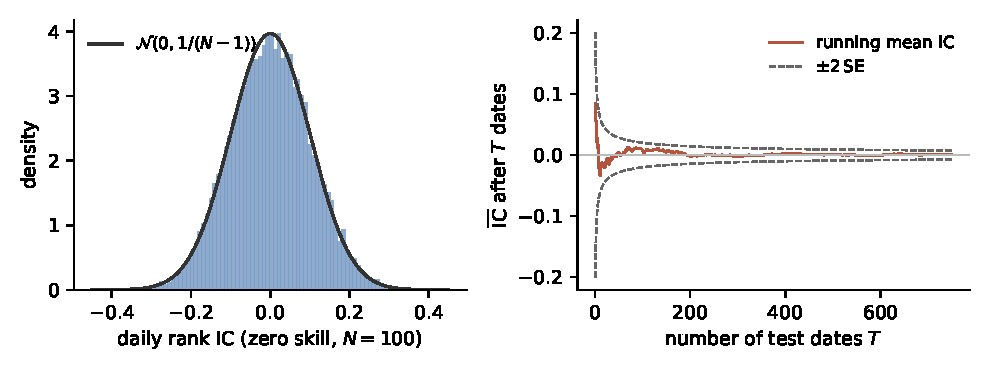
\includegraphics[width=\textwidth]{figures/null_ic.pdf}
\caption{\textbf{Zero skill produces large ICs.} Left: the simulated
distribution of the daily rank IC for a signal with no predictive content
($N=100$ names), with the $\gauss(0, 1/(N-1))$ overlay of
Proposition~\ref{prop:nullic}. Right: the running mean IC of one zero-skill
strategy over 750 test dates, against $\pm 2$ standard-error bands. Early
stretches of apparent skill (or anti-skill) of $|\ICbar| \approx 0.03$ ---
the size of a genuinely good signal --- are routine and mean nothing.}
\label{fig:nullic}
\end{figure}

\subsection{Aggregation and the arithmetic of proof}\label{sec:aggregation}

Average the daily series: $\ICbar = \frac1T \sum_t \IC_t$. If the daily ICs
were independent with standard deviation $\sigma_{\IC}$, the standard error
of the mean would be $\sigma_{\IC}/\sqrt{T}$, giving the $t$-statistic
\[
  t \;=\; \frac{\ICbar}{\sigma_{\IC}/\sqrt{T}}
    \;=\; \underbrace{\frac{\ICbar}{\sigma_{\IC}}}_{\textstyle\ICIR}
          \cdot \sqrt{T},
\]
where the ratio $\ICIR$ --- the per-date information ratio of the IC series
--- measures the signal's \emph{consistency}. This immediately yields the
book's first piece of experimental arithmetic: the number of test dates
needed before a true mean IC is statistically distinguishable from zero at
level $t^\ast$ is
\[
  T \;\geq\; \left( \frac{t^\ast \, \sigma_{\IC}}{\ICbar} \right)^{\!2}.
\]

\begin{example}\label{ex:arith}
A true $\ICbar = 0.03$ with realistic daily dispersion
$\sigma_{\IC} = 0.15$ (the null's $0.10$ plus regime-driven variation) needs
$T \ge (2 \times 0.15/0.03)^2 = 100$ test dates for $t = 2$, and $225$ dates
for $t = 3$ --- roughly five and eleven months of daily evaluation
respectively, \emph{if the daily ICs were independent}. They are not: with an
$h$-day label, adjacent dates share $h-1$ days of the outcome window, which
positively correlates the IC series and \emph{reduces} the effective $T$.
Every ``significant'' claim in this project is built to survive this
arithmetic; most published claims in the field would not.
\end{example}

\begin{engineering}[the evaluation harness]
This arithmetic is why the package's walk-forward harness
(\code{nec\_moe/evaluation.py}) pools ICs \emph{across all test dates of all
folds} before summarizing, reports $\ICbar$, $\sigma_{\IC}$, $\ICIR$ and
$t = \ICIR\sqrt{T}$ together rather than any of them alone, and why the label
overlap of Example~\ref{ex:arith} resurfaces twice: as the purging rule
(train/test separation must respect the $h$-day label span) and as a caution
against taking the nominal $t$-statistic at face value when $h > 1$.
\end{engineering}

\section{Why the problem resists standard machine learning}\label{sec:hostile}

Four properties of this environment, in increasing order of subtlety. They
are worth naming precisely, because each one dictates a specific piece of the
system built in this book.

\subsection{Noise dominates: variance is the binding constraint}

With $R^2$ of order $10^{-3}$, the mean-squared-error decomposition
\[
  \E\bigl[(\hat f(\vx) - f(\vx))^2\bigr]
  \;=\; \underbrace{\text{bias}^2}_{\text{model too simple}}
  \;+\; \underbrace{\text{variance}}_{\text{model too responsive to noise}}
\]
is wildly lopsided: the function $f$ being estimated is minuscule, while the
noise available for a flexible model to memorize is everything else. A model
class with the capacity to represent rich structure will, on a finite panel,
mostly represent noise. Concretely: a panel of $N = 500$ names over ten years
($T \approx 2{,}500$) has $1.25$ million rows, which sounds like plenty ---
until Section~\ref{sec:dependence} shreds the ``independent samples''
reading, and until one compares it with the four \emph{million} parameters of
the prototype's LSTM stack (Chapter~\ref{ch:autopsy}, defect~5). The
project's response is threefold: small encoders (a one-layer GRU with hidden
size 32, not an eight-layer LSTM), a mixture architecture whose components
are individually simple, and capacity-\emph{matched} baselines (Chapter~16)
so that any claimed advantage of the mixture cannot be an artifact of
parameter count.

\subsection{Nothing is stationary}

The mapping $\vx \mapsto y$ is not fixed. It drifts on two timescales.
Slowly: signals decay as they become known and traded away --- the
out-of-sample deterioration of published anomalies is one of the most robust
findings in empirical asset pricing (McLean and Pontiff, 2016, document
returns falling by roughly a third to a half after publication). And quickly:
the \emph{same} characteristic can predict with opposite signs in different
market states --- momentum's behavior in calm markets versus its crashes in
volatile rebounds being the canonical example, developed in detail in
Chapter~\ref{ch:regimes}. Slow drift motivates walk-forward evaluation
(train strictly on the past, test strictly on the future, refit as time
advances --- Chapter~15). Fast, recurring, state-dependent change is the
thesis itself: it motivates \emph{regime-conditional} models, in which the
cross-sectional mapping is allowed to depend on a latent market state. That
motivation is the subject of the next chapter, so here we only flag the
distinction: walk-forward handles drift you cannot model; regimes are a bet
that part of the drift is \emph{recurring structure} you can.

\subsection{Samples are deeply dependent}\label{sec:dependence}

The $1.25$ million rows above are not $1.25$ million observations in any
statistically meaningful sense.

\emph{Cross-sectionally}, names co-move through common factors: on a given
date, a large share of every stock's return is the market and industry
component. The effective number of independent observations per date is far
smaller than $N$. A back-of-envelope: if pairwise return correlations average
$\bar\rho_c$, the variance of the equal-weighted mean of $N$ names is
$\frac{\sigma^2}{N}\bigl(1 + (N-1)\bar\rho_c\bigr)$, so the effective sample
size is $N_{\text{eff}} = N / \bigl(1 + (N-1)\bar\rho_c\bigr)$; with
$\bar\rho_c = 0.25$ and $N = 500$, $N_{\text{eff}} \approx 4$ --- for
estimating the common component. Cross-sectional \emph{ranking} signals fare
better (the common component cancels between long and short legs, which is
precisely why the task is defined cross-sectionally), but the lesson stands:
row counts overstate information content by orders of magnitude.

\emph{Temporally}, overlapping $h$-day labels make adjacent dates share
outcome information (Example~\ref{ex:arith}), and features themselves are
slow-moving (today's momentum is yesterday's momentum plus a daily
increment), so consecutive rows of the design matrix are near-duplicates.

\begin{whatbreaks}[i.i.d.\ assumptions applied to panels]
Every standard tool that assumes independent samples --- cross-validation
with random splits, bootstrap standard errors, learning-curve heuristics,
early stopping on a random validation set --- silently breaks on panel data.
Random splits are the worst offender: they place rows from date $t$ in
training and rows from $t\pm1$ (near-duplicates with overlapping labels) in
validation, so validation error estimates in-sample error, model selection
overfits, and reported performance can be pure leakage. This is why the
evaluation protocol of Part~V never once splits randomly: every split in the
project is chronological, and every train/test boundary is purged by the
label horizon.
\end{whatbreaks}

\subsection{Errors are rewarded asymmetrically}\label{sec:ratchet}

The most insidious property is not statistical but sociological, and it
deserves a name.

\begin{remark}[The leakage ratchet]\label{rem:ratchet}
In most software, bugs make results worse, so testing and debugging drive
quality up. In backtesting, an entire class of bugs --- look-ahead in
features, survivorship in the universe, test data touched during tuning,
selection among many trials --- make results \emph{better}. A researcher who
debugs whatever hurts performance and leaves alone whatever helps it is
running a ratchet that converges to maximally self-deceiving code, all while
every individual action feels like diligence.
\end{remark}

The ratchet cannot be defeated by intending to be careful, because each of
its clicks is invisible at the moment it happens. It is defeated
structurally, by making the honest path the default path: features constructed
under a schema in which the target \emph{cannot} occupy a feature column
(Chapter~12); leakage stated as executable invariants rather than intentions;
evaluation code shared between the model and every baseline so the grading
cannot silently differ; every trained configuration logged to an append-only
registry so the multiplicity of Section~\ref{sec:whatisresult} cannot be
understated; and selection events (``best of $N$'') recorded as data. Part~V
and Part~VI are, in essence, a systematic dismantling of
Remark~\ref{rem:ratchet}, and it is the single most important idea in this
book that is not mathematics.

\section{What counts as a result}\label{sec:whatisresult}

Given all of the above, we can state what the project is actually obliged to
produce. Three commitments define ``a result.''

\subsection{Distributional prediction, scored properly}

The models in this book output not a point estimate but a conditional
distribution $p(y \mid \vx)$ --- for the mixture models of Part~II, a
$K$-component Gaussian mixture. Distributions are graded by the negative
log-likelihood on held-out data,
$\NLL = -\frac1n \sum_j \log p(y_j \mid \vx_j)$, which is a \emph{proper
scoring rule}: its expectation is uniquely minimized by reporting the true
conditional distribution, so a model cannot improve its grade by hedging or
exaggerating its uncertainty.

It is worth deriving what NLL means in the simplest case, because the result
recurs throughout the book. For a single Gaussian model
$p(y \mid \vx) = \gauss(y;\, \mu(\vx), \sigma^2)$,
\[
  \NLL \;=\; \frac1n \sum_j
  \left[ \tfrac12 \log(2\pi\sigma^2)
       + \frac{(y_j - \mu(\vx_j))^2}{2\sigma^2} \right],
\]
so at \emph{fixed} $\sigma$, minimizing NLL is exactly minimizing
mean-squared error --- nothing new is being asked of the mean. The new
content appears when $\sigma$ is \emph{learned}: setting
$\partial \NLL / \partial \sigma^2 = 0$ gives
$\hat\sigma^2 = \frac1n \sum_j (y_j - \mu(\vx_j))^2$, the mean squared
residual, and substituting back,
\[
  \min_{\sigma} \NLL \;=\; \tfrac12 \log \hat\sigma^2 + \tfrac12\log(2\pi) + \tfrac12 .
\]
Two consequences. First, NLL comparisons between models are (monotone
transformations of) residual-variance comparisons in this simple case, so
nothing exotic is smuggled in by switching metrics. Second --- and this is
the reason the thesis models are distributional at all --- once $\sigma$ may
depend on the regime, the model can say ``\emph{in this state, everything is
noisier},'' and the likelihood rewards it for being \emph{right about its own
uncertainty}. Chapter~2 argues that time-varying $\sigma$ is the single most
robust empirical fact about returns; a scoring rule blind to it (like raw
MSE) throws away precisely the structure the thesis is about. NLL is also
what makes the model comparison fair: the package's MLP baseline is
deliberately a single NEC expert with its own learned $\sigma$, trained on
the same Gaussian NLL, so ``mixture versus single model'' compares like with
like (Chapter~16).

\subsection{Economic significance, costed}

Statistical significance does not pay transaction costs. A result must also
survive translation into the portfolio construction it implies: the quantile
long-short of Chapter~16, with turnover measured and a cost per unit of
traded notional subtracted. A signal with a fine IC that turns over its
entire book daily can be worthless net of costs; the report that omits
turnover is not a result but an advertisement. (Per-period information
ratios are also never annualized in this project unless the dates are real
trading days and the annualization is stated --- a small honesty with a long
history of being fudged.)

\subsection{Significance that survives its own search}

Finally, the multiplicity commitment. A research project does not train one
model; it trains dozens of configurations, seeds, and variants, and reports
the ones that look best. Under the null, the maximum of $M$ independent
standard normal $t$-statistics is approximately $\sqrt{2 \ln M}$ --- with
$M = 20$ trials, expect a best $t$ of about $2.4$ \emph{from pure noise}.
``We ran many things and this one worked'' is therefore not evidence unless
the many things are counted and the threshold adjusted. The machinery ---
trial registries that make the count un-losable, false-discovery-rate
control across the claim family, the deflated Sharpe ratio, and
pre-registration of the final experiment --- is Chapter~17's subject, and it
exists because of this paragraph.

\begin{engineering}[the thesis question, made falsifiable]
The commitments above compile the vague ambition ``build a regime model that
predicts returns'' into a falsifiable protocol: \emph{does the
regime-conditional mixture beat capacity-matched single-model baselines on
held-out NLL and pooled rank-IC, under purged walk-forward evaluation, with
seeds treated as replicates, the claim family corrected for multiplicity,
and costs charged?} Every clause traces to a section of this chapter. The
rest of the book is the construction of a system that can answer the
question --- and that deserves to be believed when it does.
\end{engineering}

\begin{origins}[reading for this chapter]
The information coefficient and its aggregation arithmetic are treated in
Grinold and Kahn, \emph{Active Portfolio Management} (2000), whose
``fundamental law'' $\mathrm{IR} \approx \IC \cdot \sqrt{\text{breadth}}$ is
the industry ancestor of Section~\ref{sec:aggregation}. The out-of-sample
decay of published signals is documented by McLean and Pontiff (2016,
\emph{Journal of Finance}). The leakage ratchet and the multiplicity crisis
are the animating concerns of L\'opez de Prado, \emph{Advances in Financial
Machine Learning} (2018), whose purging/embargo constructions reappear in
Chapter~15 and whose deflated Sharpe ratio (with Bailey) is derived in
Chapter~17. Proper scoring rules go back to Brier (1950) and are surveyed by
Gneiting and Raftery (2007).
\end{origins}

\begin{codewalk}[nec\_moe/data.py --- the panel contract]
The chapter's definitions exist in code as a frozen dataclass; it is worth
seeing how directly. A \code{Panel} is five aligned tensors ---
\code{x\_seq} $(n, T_w, d_{\text{seq}})$, \code{x\_snap}
$(n, d_{\text{snap}})$, \code{y} $(n,)$, \code{date} $(n,)$, \code{entity}
$(n,)$ --- one row per (name, date) pair:

\begin{lstlisting}
@dataclass(frozen=True)
class Panel:
    x_seq: Tensor    # (n, T_w, d_seq) trailing windows
    x_snap: Tensor   # (n, d_snap)    point-in-time snapshots
    y: Tensor        # (n,)           forward return -- the ONLY
                     #                forward-looking column
    date: Tensor     # (n,)           int64 date index
    entity: Tensor   # (n,)           int64 name index
\end{lstlisting}

Three details echo the chapter. The target is a separate tensor --- there is
no ``reserved column'' inside a feature matrix for it to hide in
(Definition~\ref{def:pit}; this kills defect~7 of
Chapter~\ref{ch:autopsy} structurally). All splitting utilities are
date-based (\code{subset\_dates}, \code{split\_by\_date}) --- the API simply
does not offer a random row split, making the honest path the only paved one
(Remark~\ref{rem:ratchet}). And \code{date}/\code{entity} ride along every
batch, because per-date grading (Definition~\ref{def:ic}) and turnover
accounting need them at scoring time.
\end{codewalk}

\exercisehead

\begin{exercise}\label{ex:1-null}
(\emph{Null IC, finite-sample.}) Complete the proof of
Proposition~\ref{prop:nullic} by verifying the two permutation moments used:
for a uniformly random permutation $\Pi$ and a centered, normalized vector
$b$, show $\E[b_{\Pi(i)}^2] = 1/N$ and
$\E[b_{\Pi(i)}b_{\Pi(i')}] = -1/\bigl(N(N-1)\bigr)$ for $i \neq i'$. Then
show that as $N \to \infty$, $\sqrt{N-1}\,\IC_t$ is asymptotically standard
normal. (Hint: Hoeffding's combinatorial central limit theorem, or argue via
the projection onto simple linear rank statistics.)
\end{exercise}

\begin{exercise}\label{ex:1-quantile}
(\emph{From IC to portfolio spread.}) Suppose scores and outcomes are jointly
Gaussian across a date's cross-section with correlation $\rho$, outcomes with
standard deviation $\sigma_y$. Show the expected top-minus-bottom
\emph{quintile} spread is
$\E[\text{L}-\text{S}] = \rho\,\sigma_y\,
(\E[Z \mid Z > z_{0.8}] - \E[Z \mid Z < z_{0.2}])
\approx 2.8\,\rho\,\sigma_y$, where $Z$ is standard normal and $z_q$ its
quantiles. (Truncated-normal means: $\E[Z \mid Z > c] = \phi(c)/(1-\Phi(c))$.)
With $\rho = 0.03$ and daily cross-sectional vol $\sigma_y = 2\%$, what is
the expected daily spread in basis points, before costs?
\end{exercise}

\begin{exercise}\label{ex:1-bestofN}
(\emph{Hands-on: the ratchet in miniature.}) Using numpy, simulate $M = 20$
zero-skill strategies, each scored on $250$ dates with $N = 100$ names.
Report the best strategy's $\ICbar$, its na\"ive $t$-statistic, and how often
(over 1{,}000 repetitions) the best $t$ exceeds $2$. Compare the frequency
with the $\sqrt{2\ln M}$ heuristic of Section~\ref{sec:whatisresult}.
\end{exercise}

\begin{exercise}\label{ex:1-tstat}
(\emph{Experimental arithmetic.}) You expect $\ICbar = 0.02$ and
$\sigma_{\IC} = 0.12$. (a) How many test dates do you need for $t \geq 3$?
(b) The label horizon is $h = 5$ days; assuming the overlap makes the IC
series behave like an MA($h{-}1$) process with first-order autocorrelation
$\approx (h-1)/h$ decaying linearly to zero at lag $h$, derive the variance
inflation factor for $\ICbar$ and the corrected date count. (c) The package's
default evaluation reserves \code{n\_folds} $\times$
\code{test\_dates\_per\_fold} dates; what settings meet your corrected count
on a ten-year daily panel?
\end{exercise}

\begin{exercise}\label{ex:1-nll}
(\emph{NLL and MSE.}) (a) Verify the profiled-NLL identity
$\min_\sigma \NLL = \frac12 \log \hat\sigma^2 + \text{const}$ of
Section~\ref{sec:whatisresult}. (b) Two models have held-out NLLs $1.372$
and $1.351$ (natural logs). By what percentage do their implied residual
variances differ? (c) Explain why NLL can prefer model A over model B even
when B has lower MSE --- construct a two-point example with heteroskedastic
data.
\end{exercise}

\begin{exercise}\label{ex:1-panel}
(\emph{Hands-on: probing the contract.}) In the repository, construct a
synthetic panel via \code{SyntheticRegimePanel} (see
\code{nec\_baseline/README.md}), and (a) verify from tensor shapes that no
feature column equals the target; (b) use \code{split\_by\_date} and confirm
no training date exceeds any test date; (c) try to build a random row split
with the public \code{Panel} API and report what stops you. Read
\code{tests/test\_no\_lookahead} (Stage-B tests) and summarize, in one
paragraph, the exact invariant it pins.
\end{exercise}

\chapter{The Case for Regimes}\label{ch:regimes}

\begin{quote}\small\itshape
Chapter~\ref{ch:cross} established that the cross-sectional mapping drifts.
This chapter argues that part of the drift is not formless: markets move
between persistent, recurring \emph{states}, and the statistical footprint of
those states is visible in the most robust stylized facts about returns. We
derive that footprint (fat tails from mixing, volatility clustering from
persistence), meet the classical model built on it (Hamilton's Markov
switching), and then take the step that defines the thesis: letting the
\emph{cross-sectional prediction function itself} depend on the regime. The
chapter ends with the precise model class the rest of the book constructs,
trains, and evaluates.
\end{quote}

\section{Three stylized facts}\label{sec:facts}

Daily equity returns, at the index or single-name level, exhibit three
regularities so stable across markets and decades that any credible model
must account for them:

\begin{enumerate}[label=(F\arabic*),leftmargin=2.2em]
\item \emph{Fat tails.} Return distributions have far more mass in their
  tails than a Gaussian of the same variance. Sample excess kurtosis of daily
  index returns is typically in the range $5$--$30$ (a Gaussian has $0$);
  multi-sigma days occur orders of magnitude more often than normality
  predicts.
\item \emph{Volatility clustering.} Large-magnitude days follow
  large-magnitude days: the autocorrelation of $|r_t|$ and $r_t^2$ is
  positive and decays slowly over weeks to months, even while the
  autocorrelation of $r_t$ itself is negligible. Mandelbrot's 1963
  formulation stands: ``large changes tend to be followed by large changes,
  of either sign, and small changes by small changes.''
\item \emph{State-dependent relationships.} Correlations between assets rise
  sharply in stressed markets, and --- most important for this thesis ---
  the \emph{predictive content of cross-sectional characteristics changes
  with the market state}. Section~\ref{sec:conditional} develops the
  canonical example.
\end{enumerate}

The regime hypothesis is a single explanation for all three: returns are
conditionally simple (say, Gaussian) given a latent market state $S_t$, the
state modulates the parameters (above all the volatility), and the state is
\emph{persistent}. The next section shows this is not hand-waving --- the
first two facts follow \emph{mathematically} from exactly that structure.

\section{Mixtures generate the stylized facts}\label{sec:mixmath}

\subsection{Fat tails from mixing}

Consider the simplest regime model: each day belongs to state
$k \in \{1, \dots, K\}$ with probability $p_k$, and conditional on the state
the return is centered Gaussian with state-specific volatility,
$r \mid S = k \sim \gauss(0, \sigma_k^2)$. The unconditional law is the
\emph{scale mixture} $r \sim \sum_k p_k \gauss(0, \sigma_k^2)$.

\begin{proposition}[Scale mixtures are leptokurtic]\label{prop:kurtosis}
Let $r$ follow the scale mixture above and write
$m_2 = \sum_k p_k \sigma_k^2$ for its variance. Then its kurtosis is
\[
  \kappa \;=\; \frac{\E[r^4]}{\E[r^2]^2}
  \;=\; 3\,\frac{\sum_k p_k \sigma_k^4}{\bigl(\sum_k p_k \sigma_k^2\bigr)^2}
  \;\geq\; 3,
\]
with equality if and only if all the $\sigma_k$ with $p_k > 0$ are equal.
\end{proposition}

\begin{proof}
Condition on the state and use Gaussian moments
($\E[r^2 \mid S{=}k] = \sigma_k^2$, $\E[r^4 \mid S{=}k] = 3\sigma_k^4$):
\[
  \E[r^2] = \sum_k p_k \sigma_k^2, \qquad
  \E[r^4] = 3 \sum_k p_k \sigma_k^4 .
\]
Let $V$ be the random variable taking value $\sigma_k^2$ with probability
$p_k$ (the ``randomized variance''). Then
$\kappa = 3\,\E[V^2] / (\E[V])^2$, and by Jensen's inequality (or
Cauchy--Schwarz) $\E[V^2] \ge (\E[V])^2$, with equality iff $V$ is almost
surely constant.
\end{proof}

The inequality carries a reading worth memorizing: \emph{excess kurtosis is
the variance of the variance}. Precisely,
$\kappa - 3 = 3\,\Var(V)/(\E V)^2$ --- unconditional fat tails are what
time-varying (here: state-varying) volatility looks like after the state is
integrated out. A two-state example calibrated to the package's synthetic
defaults, $\sigma = (0.5, 2.5)$ with equal weights: $\E V = 3.25$,
$\E V^2 = 19.56$, so $\kappa = 3 \times 19.56 / 3.25^2 \approx 5.6$ ---
nearly double the Gaussian's $3$, from conditional normality alone. And the
\emph{proportions} matter as much as the levels: the same $5\times$
volatility ratio concentrated in a \emph{rare} turbulent state (weight
$\approx 4\%$) drives $\kappa$ above $20$, squarely into the empirical
range --- Exercise~\ref{ex:2-kurt} derives the optimal rarity. Fat tails
are the signature of occasional, distinct turbulence, not of two
similar-sized populations. Figure~\ref{fig:regimes} (bottom left) shows the
effect on a log-density scale: the mixture's tails sit far above the
moment-matched Gaussian's.

The moral for modeling: one does not need heavy-tailed \emph{conditional}
distributions to reproduce heavy-tailed data. A mixture of Gaussians with
state-dependent $\sigma_k$ --- exactly the emission structure of the thesis
model --- generates realistic tails while keeping every component
analytically tractable. (This is also the honest reading of ``Gaussian
assumption'' criticisms: the model class is only conditionally Gaussian; its
unconditional predictions are not.)

\begin{figure}[t]
\centering
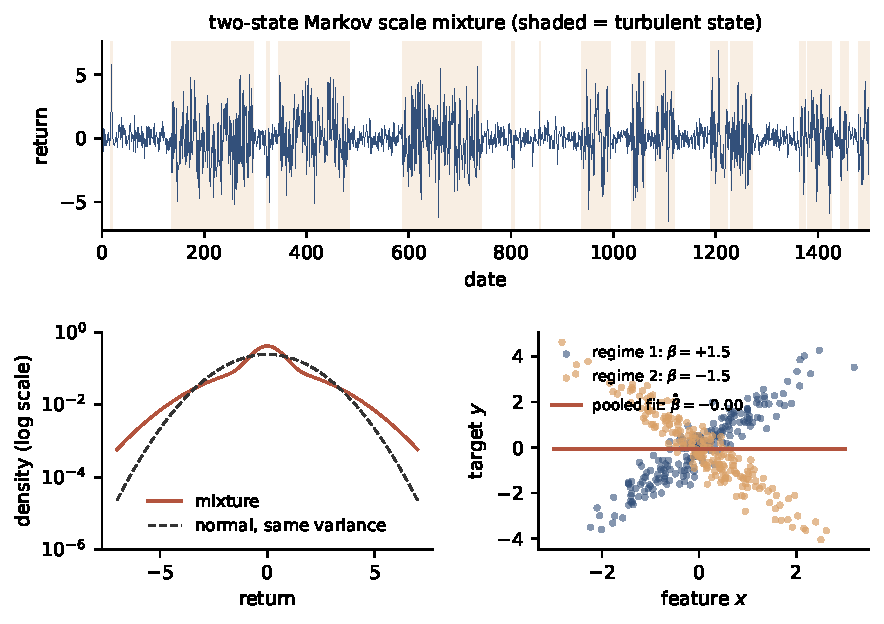
\includegraphics[width=\textwidth]{figures/regimes.pdf}
\caption{\textbf{Regimes generate the stylized facts.} Top: a return series
from a two-state Markov scale mixture ($\sigma = (0.6, 2.2)$, stay
probability $0.98$); turbulent-state periods shaded. Volatility clustering
is visible to the naked eye --- and provably absent if the same states are
shuffled i.i.d. Bottom left: the unconditional density against a Gaussian
of identical variance (log scale) --- fat tails from
Proposition~\ref{prop:kurtosis}. Bottom right: the sign-flip construction of
Section~\ref{sec:signflip} --- two regimes with slopes $\pm\beta$; the
pooled fit (red) estimates $\hat\beta \approx 0$ and is structurally blind
to a relationship that is perfectly strong within each regime.}
\label{fig:regimes}
\end{figure}

\subsection{Clustering requires persistence}\label{sec:persistence}

Fact (F1) needed only a \emph{mixture}. Fact (F2) --- clustering --- needs
more: it is a statement about \emph{dependence over time}, and an i.i.d.\
state sequence cannot produce it. If $S_t$ is drawn independently each day,
then $r_t^2$ and $r_{t+s}^2$ are independent for $s \ge 1$, so
$\Corr(r_t^2, r_{t+s}^2) = 0$: an i.i.d.\ mixture has fat tails but no
memory. Clustering is evidence that the state \emph{persists}.

The minimal persistent-state model is a Markov chain. Let $S_t$ be a
two-state chain with stay probabilities $a = \Prob(S_{t+1}{=}1 \mid S_t{=}1)$
and $b = \Prob(S_{t+1}{=}2 \mid S_t{=}2)$, and $r_t = \sigma_{S_t}\,
\varepsilon_t$ with $\varepsilon_t$ i.i.d.\ standard normal.

\begin{proposition}[Squared-return autocorrelation]\label{prop:acf}
Under the two-state Markov scale mixture, for lags $s \geq 1$,
\[
  \Corr\bigl(r_t^2,\; r_{t+s}^2\bigr)
  \;=\; c \cdot \lambda^{s},
  \qquad \lambda = a + b - 1,
\]
where $c \in (0, 1)$ is a constant depending on
$(a, b, \sigma_1, \sigma_2)$ but not on $s$. The chain's second eigenvalue
$\lambda$ --- its persistence --- is the decay rate of volatility
clustering.
\end{proposition}

\begin{proof}
Write $v_t = \sigma^2_{S_t}$, so $r_t^2 = v_t \varepsilon_t^2$ with
$\varepsilon_t^2$ i.i.d., mean $1$, independent of the state path. Then for
$s \ge 1$, $\Cov(r_t^2, r_{t+s}^2) = \Cov(v_t, v_{t+s})$ (the independent
$\varepsilon^2$ factors contribute $\E[\varepsilon^2]^2 = 1$ across distinct
times), while $\Var(r_t^2) = \E[v_t^2]\E[\varepsilon^4] - \E[v_t]^2 =
3\E[v_t^2] - \E[v_t]^2 > \Var(v_t)$; hence the correlation of $r^2$ is a
fixed positive multiple $c < 1$ of the correlation of $v$. It remains to
compute $\Corr(v_t, v_{t+s})$. The transition matrix
$A = \bigl(\begin{smallmatrix} a & 1-a \\ 1-b & b \end{smallmatrix}\bigr)$
has eigenvalues $1$ and $\lambda = a + b - 1$; its stationary distribution
is $\bar\pi = \bigl(\frac{1-b}{2-a-b}, \frac{1-a}{2-a-b}\bigr)$. For a
two-state chain, any function $f(S_t)$ --- here $v_t$, which takes two
values --- has autocorrelation exactly $\lambda^s$: decompose $f$ into its
stationary mean plus a component along the second left-eigenvector; the
$s$-step transition operator scales that component by $\lambda^s$, and
correlations are invariant to the affine part. Therefore
$\Corr(v_t, v_{t+s}) = \lambda^s$ and
$\Corr(r_t^2, r_{t+s}^2) = c\,\lambda^s$.
\end{proof}

With stay probabilities $a = b = 0.98$ (mean regime duration
$1/(1-a) = 50$ days), $\lambda = 0.96$: squared-return autocorrelations
decay by only $\sim\!4\%$ per day and remain visible for months ---
matching (F2). The top panel of Figure~\ref{fig:regimes} is this process,
and the clustering is unmistakable.

Two lessons transfer directly to the thesis model. First, \emph{persistence
is where the memory lives}: the conditional distribution of $r_t$ given the
state needs no dependence structure at all; the Markov chain carries all of
it. This division of labor --- simple emissions, dynamic state --- is
exactly the architecture of Part~II's models. Second, mean regime duration
$1/(1-a)$ gives persistence an interpretable scale, which will return in
Part~III as a \emph{persistence-biased initialization}: the learned
transition matrix is initialized sticky ($a$ near $0.9$--$0.98$), encoding
the prior belief that regimes last weeks, not hours.

\begin{origins}[Hamilton 1989 and what came before]
Mixture-of-normals descriptions of speculative prices go back to Mandelbrot
(1963) and Fama (1965) on fat tails, and to Clark (1973), whose subordinated
process --- returns as Gaussians with a randomized variance --- is
Proposition~\ref{prop:kurtosis} in continuous form. Engle's ARCH (1982) and
Bollerslev's GARCH (1986) capture clustering with an observable, recursively
defined variance. The regime-switching alternative is due to James D.
Hamilton, ``A New Approach to the Economic Analysis of Nonstationary Time
Series and the Business Cycle'' (\emph{Econometrica}, 1989): an
autoregression whose parameters switch according to an unobserved two-state
Markov chain, estimated on U.S.\ GNP growth, with the states identified
ex post as expansions and recessions --- NBER-dated recessions were
recovered by the filter without ever being shown to it. Hamilton's technical
contribution is the estimation machinery: because the state is latent, the
likelihood must integrate over all state paths, which his \emph{forward
filter} accomplishes recursively in $O(TK^2)$. That filter --- and the
distinction between filtering ($\Prob(S_t \mid \text{data up to } t)$),
which is causal, and smoothing ($\Prob(S_t \mid \text{all data})$), which
is not --- is derived in full in Chapter~7 and sits verbatim inside the
thesis model's HMM gate. The classical Hamilton model itself survives in the
package as \code{ExpertConfig(kind="classical")} $\times$
\code{PriorConfig(kind="hmm")}: constant per-regime Gaussians under a
learned Markov prior, used as a parameter-recovery test bed and an honest
classical baseline.
\end{origins}

\section{From marginal regimes to conditional regimes}\label{sec:conditional}

Everything so far concerned the \emph{marginal} distribution of returns ---
enough for risk modeling, but not yet a prediction model. The thesis takes
one further step, and it is the step that turns regime modeling into
cross-sectional alpha research:

\begin{center}
\emph{Let the map from characteristics to expected returns\\
depend on the regime.}
\end{center}

\subsection{The economics: momentum as the canonical example}

Fact (F3) is best seen through the best-documented cross-sectional signal:
momentum (buy the past year's winners, short the losers; Jegadeesh and
Titman, 1993). Its average profitability is among the most replicated
findings in finance --- and so are its \emph{crashes}. Daniel and Moskowitz
(``Momentum crashes,'' \emph{JFE}, 2016) document that momentum's worst
episodes are concentrated in a specific, identifiable state: panic markets
--- high volatility, following a market decline --- especially at the turn
into a sharp rebound. In 1932 and 2009, the losers-rebound effect was so
violent that the strategy lost most of a century's compounding in weeks. In
the language of this book: the coefficient linking the momentum
characteristic to expected return is positive in calm states and
\emph{negative} in high-volatility rebound states. Similar state-dependence
is documented for reversal strength, size, quality, and the
low-vol anomaly; regime-dependent factor performance is the working
assumption of practitioner asset allocation.

For prediction, this is qualitatively different from (F1)--(F2). A signal
whose \emph{sign flips} with the state is invisible to any model that
assumes one global mapping --- not weakened, \emph{invisible}, as the next
subsection makes exact.

\subsection{The statistics: what pooling destroys}\label{sec:signflip}

Idealize the situation. Two regimes, equally likely; within regime $k$ the
cross-section obeys a linear model with regime-dependent slope:
\[
  y_i \;=\; \beta_{S}\, x_i + \varepsilon_i,
  \qquad
  \beta_1 = +\beta,\;\; \beta_2 = -\beta,
  \qquad
  \varepsilon_i \sim \gauss(0, \sigma_\varepsilon^2),
\]
with $x_i$ standardized and independent of the regime. What does the best
\emph{global} (regime-blind) model do?

\begin{proposition}[Pooling annihilates a sign-flipping signal]
\label{prop:signflip}
Under the model above, the population regression of $y$ on $x$, pooled over
regimes, has slope
\[
  \beta_{\mathrm{pool}}
  = \frac{\Cov(y, x)}{\Var(x)}
  = \E[\beta_S]
  = \tfrac12 \beta + \tfrac12 (-\beta) = 0 ,
\]
and the pooled model's cross-sectional $R^2$ --- hence its IC --- is zero.
An oracle that knows $S$ attains
$R^2 = \beta^2 / (\beta^2 + \sigma_\varepsilon^2)$ in every regime.
Moreover, no measurable function $f(x)$ of the characteristic alone can do
better than the pooled slope: $\E[y \mid x] = \E[\beta_S]\,x = 0$ for all
$x$.
\end{proposition}

\begin{proof}
$\Cov(y, x) = \E[\beta_S x^2] + \E[\varepsilon x] = \E[\beta_S]\E[x^2]$
by independence of $S$ and $x$ and exogeneity of $\varepsilon$; the last
claim is the tower property: $\E[y \mid x] = \E[\E[y \mid x, S] \mid x] =
x\,\E[\beta_S] = 0$.
\end{proof}

The final clause is the sharp one: the failure is not linearity. \emph{Any}
model --- a gradient-boosted forest, a deep network --- that consumes only
the characteristic has zero predictive content in this world, because the
conditional mean given the characteristic alone is identically zero. The
information is real (the oracle's $R^2$ can be near $1$) but it lives
entirely in the \emph{interaction} between the characteristic and the state.
Figure~\ref{fig:regimes} (bottom right) draws the picture: two clean
regressions of slope $\pm 1.5$; one flat, useless pooled line.

This construction is deliberately extreme --- real regime-dependence is a
matter of degree, attenuation rather than annihilation (if regime
probabilities are $p \ne \tfrac12$ or slopes merely shrink, the pooled slope
is $\E[\beta_S] \ne 0$ and pooling loses part of the signal). But its
extremity is precisely what makes it \emph{useful}: it is the ideal
\textbf{planted truth} for testing a regime model. In a world generated by
Proposition~\ref{prop:signflip}, a working regime-conditional model must
achieve high IC while every regime-blind baseline must, by mathematics
rather than by luck, achieve none. The package's synthetic panel generator
implements exactly this world, and the claim ``the mixture beats the pooled
baseline \emph{here}'' is enforced as a permanent regression test --- both
directions of it (the baselines must also \emph{win} on a no-regime world,
proving they are not straw men). Chapter~14 builds the instrument; the walk-through
below shows its heart.

\begin{whatbreaks}[if regimes are real and the model is global]
Proposition~\ref{prop:signflip} is the precise content of the claim
``non-stationarity is not just drift'' from
Section~\ref{sec:hostile}. Where relationships flip with the state, a global
model does not degrade gracefully --- it averages the states and reports
noise. Worse, it does so \emph{silently}: the fit succeeds, the loss
decreases, the diagnostics look ordinary; only the out-of-sample IC hovers
at zero. If a rich global model is given extra capacity it will typically
\emph{overfit within-sample noise} before it discovers a state interaction
it has no features to express. The failure mode is invisible without a
regime-aware alternative to compare against --- one of the quieter reasons
to build the mixture even if one ultimately bets against it.
\end{whatbreaks}

\subsection{Why not just add state features?}\label{sec:whynotfeatures}

Proposition~\ref{prop:signflip} shows the model must see \emph{some} state
information. The obvious cheap fix: append a state proxy (VIX, trailing
market volatility) as a feature to a global model, and let it learn the
interaction, e.g.\ $\hat y = g(x, v)$. With enough capacity, $g$ can
represent $\beta(v)\,x$; a universal approximator handles it in principle.
Why, then, an explicit mixture? Four reasons, in increasing order of
importance to the thesis:

\begin{enumerate}[leftmargin=2em]
\item \emph{Statistical structure.} The mixture encodes the hypothesis as
  \emph{a small number of discrete states, each with a full, simple
  cross-sectional model, plus persistence in the state process}. A generic
  interaction model must discover discreteness, persistence, and the
  within-state models from scratch, spending capacity (hence variance ---
  Section~\ref{sec:hostile}) on what the mixture gets as inductive bias. In
  a domain where variance is the binding constraint, inductive bias is not a
  convenience; it is the budget.
\item \emph{Distributional honesty.} The mixture is a model of
  $p(y \mid \vx)$ with state-dependent $\sigma_k$ --- it natively expresses
  ``high-vol state $\Rightarrow$ wider predictive distribution,'' which is
  (F1)--(F2) speaking, and it is graded on it via NLL
  (Section~\ref{sec:whatisresult}). A point-prediction interaction model
  expresses none of this.
\item \emph{The state is latent.} VIX is a proxy, not the state. A mixture
  with a learned gate can \emph{infer} the state from inputs (and, in the
  HMM variant, from its own recent posterior --- carrying the persistence of
  Section~\ref{sec:persistence} into inference). Hamilton's central lesson
  applies: treat the state as unobserved and integrate over it, rather than
  hard-coding a proxy.
\item \emph{Falsifiability.} This is the decisive one for a thesis. In the
  mixture, the state is an explicit object: one can ask ``do the learned
  regimes correspond to anything real?'' and answer by correlating the
  gate's inferred posterior with \emph{held-out} state proxies it never saw
  in training (the alignment analysis of Chapter~18's practicum
  cousin, Stage~C). In a monolithic $g(x, v)$, the regime hypothesis is
  smeared across weights, and no such question can be asked. Crucially, this
  requires the gate to be \emph{unsupervised} --- the moment one trains the
  gate to predict VIX, ``the model discovered volatility regimes'' becomes
  circular. That is Decision~B of Part~III, made here, in the theory, before
  any code.
\end{enumerate}

The honest counterpoint is also worth recording: the mixture buys these
properties at the price of a harder optimization landscape (multimodality,
symmetric local optima --- Chapter~8), an identifiability problem (labels
can permute --- Chapters~7--8), and more machinery to get wrong. The
prototype of Chapter~\ref{ch:autopsy} is what ``more machinery to get
wrong'' looks like in practice. The thesis is precisely the wager that the
structure is worth its optimization cost --- and Part~V exists so that the
wager is settled by evidence rather than by enthusiasm.

\section{The model class}\label{sec:modelclass}

We can now write down the object this book builds. Everything later --- the
loss (Chapter~5), the routing variants (Chapter~6), the HMM gate
(Chapter~7), the architecture (Part~III), the evaluation (Part~V) --- is
this definition, taken seriously.

\begin{definition}[Regime-conditional mixture of experts]\label{def:nec}
For a name--date pair with features
$\vx = (\vx^{\text{seq}}, \vx^{\text{snap}})$, the model is the conditional
mixture
\[
  p(y \mid \vx)
  \;=\; \sum_{k=1}^{K} \pi_k \,\gauss\!\bigl(y;\; \mu_k(\vx),\, \sigma_k^2\bigr),
\]
with three learned ingredients:
\begin{itemize}[leftmargin=2em]
\item \textbf{Experts} $\mu_k(\cdot)$: $K$ regime-specialized prediction
  functions (small MLPs on the snapshot features; or constants, recovering
  the classical Hamilton emission), each with its own volatility
  $\sigma_k$;
\item \textbf{A gate}, producing the mixture weights from the encoded
  sequence state $\vh = \mathrm{enc}(\vx^{\text{seq}})$;
\item \textbf{A prior mechanism} $\vpi = \mathrm{prior}(\vz, \cdot)$
  turning the gate's logits $\vz(\vh)$ into weights --- \emph{pluggable}:
  a memoryless softmax $\pi_k \propto e^{z_k}$ (and its uniform / hard /
  top-$k$ / annealed variants) for thesis Variation~2, or a causal Markov
  filter $\pi_{t,k} \propto \sum_j A_{jk}\, r_{t-1,j}$ carrying yesterday's
  posterior through a learned transition matrix for Variation~3.
\end{itemize}
Training maximizes the likelihood of held-out-able data --- equivalently,
minimizes $\NLL = -\frac1n\sum \log p(y \mid \vx)$ --- with the latent state
never observed and the gate never supervised.
\end{definition}

Each clause of Definition~\ref{def:nec} answers to a section of these first
two chapters. Conditional Gaussians with per-regime $\sigma_k$: fat tails
and honest uncertainty (Proposition~\ref{prop:kurtosis},
\S\ref{sec:whatisresult}). Regime-indexed $\mu_k(\vx)$: the sign-flip
argument (Proposition~\ref{prop:signflip}). A latent, unsupervised state
inferred by a gate: \S\ref{sec:whynotfeatures}. A pluggable prior with a
Markov option: persistence (Proposition~\ref{prop:acf}) and Hamilton's
filter. Small experts on snapshot features, a small encoder for the state:
the variance budget of \S\ref{sec:hostile}. Nothing in the model is
unmotivated; that is what a design derived from theory looks like, and
Part~III will hold the implementation to it.

\begin{codewalk}[nec\_moe/data.py --- the planted world]
The synthetic generator is Proposition~\ref{prop:signflip} plus
Proposition~\ref{prop:acf} in about a page of code. Its spec exposes exactly
the theory's knobs:

\begin{lstlisting}
@dataclass(frozen=True)
class SyntheticSpec:
    n_regimes: int = 2
    regime_process: str = "iid"    # "iid" | "markov"
    transition_stay: float = 0.95  # Markov persistence  (Prop 2.2)
    vol_levels: tuple = (0.5, 2.5) # sigma_k             (Prop 2.1)
    beta_scale: float = 1.0        # +/- beta sign flip  (Prop 2.3)
    noise_std: float = 0.5         # sigma_eps
    seed: int = 0
\end{lstlisting}

Per date, one regime $S_t$ is drawn (i.i.d.\ or sticky-Markov); every name's
target is $y_{i,t} = \beta_{S_t}^\top \vx^{\text{snap}}_{i,t} +
\sigma_{S_t}\,\varepsilon_{i,t}$ with $\beta_2 = -\beta_1$ --- the sign
flip. The sequence features carry a volatility footprint of the regime, so
the state is \emph{inferable but not given}. Because the generator also
returns the true $S_t$, tests can score regime recovery directly. The two
process modes matter later: \code{"iid"} suffices for the memoryless models
of Variation~2, while \code{"markov"} plants the persistence that the HMM
gate of Variation~3 must (and, in the tests, provably does) exploit.
\end{codewalk}

\exercisehead

\begin{exercise}\label{ex:2-kurt}
(\emph{Kurtosis, quantitatively.}) (a) Show
$\kappa - 3 = 3\,\Var(V)/(\E V)^2$ where $V$ is the randomized variance of
Proposition~\ref{prop:kurtosis}. (b) For the two-state case with weights
$(p, 1{-}p)$ and volatilities $(\sigma_1, \sigma_2)$, find the weight $p$
maximizing $\kappa$ at fixed $\sigma_2/\sigma_1 = 5$, and comment: why do
\emph{rare} volatile regimes generate the fattest tails? (c) Real daily
index returns show $\kappa \approx 10$--$30$, the equal-weight two-state
model of this chapter gives $\kappa \approx 5.6$, and your answer to (b)
exceeds $20$ with the same $5\times$ volatility ratio. What do these three
numbers together suggest about how much of empirical kurtosis regime
switching can explain, and about what the regime \emph{proportions} must
look like for it to do so?
\end{exercise}

\begin{exercise}\label{ex:2-acf}
(\emph{Persistence and memory.}) (a) Complete the proof of
Proposition~\ref{prop:acf} by computing the constant $c$ explicitly for
$a = b$: show
$c = \dfrac{\Var(v)}{3\E[v^2] - (\E v)^2}$ with
$v \in \{\sigma_1^2, \sigma_2^2\}$ equally likely, and evaluate $c$ and the
lag-10 autocorrelation for $\sigma = (0.6, 2.2)$, $a = 0.98$. (b) Show that
mean regime duration is geometric with mean $1/(1-a)$. (c) An
econometrician fits a GARCH(1,1) to data generated by this model. Which
GARCH parameter will absorb $\lambda$? (No proof --- one paragraph of
reasoning.)
\end{exercise}

\begin{exercise}\label{ex:2-pool}
(\emph{Pooling, beyond the symmetric case.}) Generalize
Proposition~\ref{prop:signflip}: regimes with probabilities $(p, 1{-}p)$
and slopes $(\beta_1, \beta_2)$. (a) Find $\beta_{\mathrm{pool}}$ and the
pooled $R^2$ as functions of $(p, \beta_1, \beta_2, \sigma_\varepsilon)$.
(b) Show the pooled model's \emph{residual variance} exceeds the oracle's by
$\Var(\beta_S)\,\E[x^2]$ --- regime dispersion in slopes reappears as
irreducible-looking noise. (c) Connect (b) to
Proposition~\ref{prop:kurtosis}: in what precise sense is ``variance of the
slope'' the cross-sectional analogue of ``variance of the variance''?
\end{exercise}

\begin{exercise}\label{ex:2-modes}
(\emph{When is a mixture visibly a mixture?}) For the equal-weight,
equal-variance two-component mixture
$\tfrac12\gauss(\mu_1, \sigma^2) + \tfrac12\gauss(\mu_2, \sigma^2)$, show
the density is bimodal if and only if $|\mu_1 - \mu_2| > 2\sigma$.
(Reduce to $f(x) \propto \cosh(\delta x)e^{-x^2/2}$ form and study its
critical points.) Conclude: regime structure can be strong yet invisible in
the marginal density --- which is why Chapter~14's planted-truth tests grade
models on \emph{recovery of the latent state}, never on eyeballing
histograms.
\end{exercise}

\begin{exercise}\label{ex:2-hands}
(\emph{Hands-on: verify the theory against the generator.}) Using
\code{SyntheticRegimePanel} with the defaults of the code walkthrough:
(a) simulate $50{,}000$ dates of the \code{"markov"} process
(\code{transition\_stay}=0.98) and verify Proposition~\ref{prop:kurtosis}'s
kurtosis and Proposition~\ref{prop:acf}'s geometric ACF decay numerically
(log-ACF should be linear in lag with slope $\log\lambda$);
(b) regress $y$ on the snapshot features pooled versus within-regime (the
generator exposes true regimes) and reproduce
Proposition~\ref{prop:signflip}'s zero-versus-oracle contrast;
(c) switch to \code{regime\_process="iid"} and confirm the ACF flattens
while the kurtosis survives --- the cleanest possible demonstration that
tails come from \emph{mixing} but memory comes from \emph{persistence}.
\end{exercise}

\chapter{Autopsy of a Prototype}\label{ch:autopsy}

\begin{quote}\small\itshape
The project did not begin with a blank page. It began with a working ---
running, loss-decreasing, plausible-looking --- prototype that was wrong in
eight distinct ways, none of which produced an error message. This chapter
dissects it. The point is not self-flagellation: the prototype's
\emph{architectural idea} was sound, and the corrected system keeps it. The
point is that each defect is a specimen of an entire \emph{class} of failure,
and the corrected system is best understood as eight class-level defenses.
Every later chapter of this book repairs something that dies on this table.
\end{quote}

\section{The specimen}\label{sec:specimen}

The prototype (preserved untouched in the repository at
\code{OP model/nec/nec\_hybrid\_explained.py}) implements a
\emph{normal-versus-extreme conditional} model --- NEC --- in three pieces:

\begin{itemize}[leftmargin=2em]
\item \code{C\_L}: a stacked LSTM sequence encoder (defaults: hidden size
  $256$, \emph{eight} layers) reading the feature window;
\item \code{C\_F}: a classifier head on one selected time step of the LSTM
  output --- \code{Linear} $\to$ \code{BatchNorm1d} $\to$ activation $\to$
  \code{Linear} $\to$ \code{nn.Softmax} --- emitting probabilities over
  \emph{three} market classes;
\item two \code{NEC\_MLP} regressors, ``\code{extreme}'' and
  ``\code{normal},'' each reading a raw slice of the input window.
\end{itemize}

The forward pass routes hard:

\begin{lstlisting}
prob  = self.classifier(h)               # (B, 3) softmax output
e_out = self.extreme(x[:, -1, :-1])      # slice: last step, drop last col
n_out = self.normal(x[:, -1, :-1])
pred  = torch.where(torch.argmax(prob, dim=1) == 1, e_out, n_out)
\end{lstlisting}

Figure~\ref{fig:prototype} draws the whole machine with the defects marked
where they live.

\begin{figure}[t]
\centering
\begin{tikzpicture}[
  font=\small,
  box/.style={draw, rounded corners=1.5pt, minimum height=8mm,
              minimum width=26mm, align=center, fill=white},
  bad/.style={draw=breakframe, circle, fill=breakbg, inner sep=1pt,
              font=\bfseries\footnotesize, text=breakframe},
  arr/.style={-{Latex[length=2mm]}, thick},
  ]
  \node[box] (xseq) {window $x$\\ $(B, T, d)$};
  \node[box, right=12mm of xseq] (lstm) {\code{C\_L}: LSTM\\ $n{=}256$, $L{=}8$};
  \node[box, right=12mm of lstm] (cf) {\code{C\_F}: head\\ BatchNorm $\to$ Softmax};
  \node[box, right=12mm of cf] (route) {\code{argmax} $=1$?};
  \node[box, below=13mm of xseq] (slice) {\code{x[:, -1, :-1]}\\ raw last-step slice};
  \node[box, below=13mm of cf] (ext) {\code{extreme} MLP};
  \node[box, below=8mm of ext] (norm) {\code{normal} MLP};
  \node[box, below=13mm of route] (pred) {$\hat y$ (one expert,\\ winner takes all)};

  \draw[arr] (xseq) -- (lstm);
  \draw[arr] (lstm) -- (cf);
  \draw[arr] (cf) -- (route);
  \draw[arr] (xseq) -- (slice);
  \draw[arr] (slice.east) -- (ext.west);
  \draw[arr] (slice.east) -- (norm.west);
  \draw[arr] (ext.east) -- (pred.west);
  \draw[arr] (norm.east) -| (pred.south);
  \draw[arr] (route) -- (pred);

  \node[bad, above right=-1.5mm and -3mm of lstm] {5};
  \node[bad, above right=-1.5mm and -3mm of cf] {3,4};
  \node[bad, above right=-1.5mm and -3mm of route] {1,2};
  \node[bad, below right=-1.5mm and -3mm of slice] {6,7};
  \node[bad, above left=-1.5mm and -2mm of lstm] {8};
\end{tikzpicture}
\caption{\textbf{The prototype, with defects in place.} Numbers key to the
ledger of Section~\ref{sec:ledger}. Note the two load-bearing absurdities
visible even at block-diagram level: the gradient cannot cross the
\code{argmax} (1), so the entire left half of the diagram --- the
four-million-parameter encoder and its head --- receives no training signal
from the prediction task; and the experts read a raw, undocumented slice of
the input (6, 7), so the encoder's summary influences \emph{nothing} except
the untrainable routing decision.}
\label{fig:prototype}
\end{figure}

Before the knife comes out, record what is \emph{right}. The prototype's
thesis --- encode the recent sequence into a state, classify the market
regime from that state, and route to a regime-specialized regressor --- is
exactly Definition~\ref{def:nec}. The corrected system keeps this skeleton
wholesale: encoder $\to$ gate $\to$ experts. Diagnosing which part of a
broken system is sound is as much a skill as finding the breaks; the ledger's
verdict on the architecture was \emph{keep}, and the whole project is
downstream of that judgment call being correct.

\section{The ledger}\label{sec:ledger}

Eight defects, in logical rather than severity order. For each: what the
code does, why it is wrong (with the mathematics where mathematics is the
right scalpel), and the repair --- with a pointer to the chapter that builds
it properly.

\subsection*{Defect 1 --- \code{argmax} routing: the gate cannot learn}

The routing decision \code{torch.where(argmax(prob) == 1, e\_out, n\_out)}
selects one expert per sample. As a function of the classifier's parameters
$\theta$, the selection $\ind{\argmax_k \mathrm{prob}_k(\theta) = 1}$ is
piecewise constant: small perturbations of $\theta$ leave the argmax
unchanged almost everywhere, so
\[
  \frac{\partial\, \hat y}{\partial \theta} = 0
  \quad \text{almost everywhere.}
\]
Autograd dutifully computes this zero. Whatever loss is attached to
$\hat y$, \emph{no gradient ever reaches the classifier} through the routing
path --- the gate's weights receive exactly zero training signal from the
prediction task. The four-million-parameter encoder feeding it is trained,
if at all, only by whatever auxiliary classification loss the gate carries,
and the routing quality can never improve from prediction feedback. Nothing
crashes; the loss on the experts still decreases; the model ``trains.''

The repair (Chapter~5) is to stop making a decision and start mixing:
weight each expert's \emph{density} by a probability and maximize the
mixture likelihood. The gradient of that objective with respect to the gate
logits will turn out to be the beautiful $\pi - r$ --- prior minus posterior
--- restoring a rich training signal to precisely the module that had none.
The lesson generalizes far beyond this file:
\begin{center}
\emph{hard decisions inside a differentiable model are gradient graves;}\\
\emph{make the decision soft, or move it outside the training path.}
\end{center}
And the story has a coda that will recur in Chapter~6: the ``obvious'' soft
fix of renormalizing the top-1 weight is \emph{equally} gradient-dead --- a
constant $1$ is as flat as an indicator --- a fact the corrected package
enforces with a validation error and proves with a test.

\subsection*{Defect 2 --- three classes collapsed to one bit}

The classifier emits three market classes; the routing consumes only
$\ind{\text{class} = 1}$. Classes $0$ and $2$ --- presumably ``calm'' and
some third state --- are silently merged, the distinction the classifier
spends capacity learning is discarded, and the number of regimes is
hard-wired into an equality test buried in the forward pass. $K$ is not a
parameter; it is folklore.

The repair is structural, not cosmetic: \emph{all} $K$ components enter the
likelihood with their own weights and densities (Chapter~5), $K$ lives in
one configuration field, and no class index has hardcoded meaning anywhere
--- which later forces an honest confrontation with the fact that mixture
components are exchangeable (the label-permutation problem, Chapters~7--8),
a problem the prototype never met only because it had welded the labels to
the furniture.

\subsection*{Defect 3 --- \code{nn.Softmax} inside the model, feeding a
second loss}

The head ends in \code{nn.Softmax}, so downstream code sees probabilities,
and any classification loss must be computed as
$\log(\mathrm{softmax}(z))$ in two separate steps. Two distinct failures
hide here. \emph{Numerical:} $\log(\mathrm{softmax}(z))$ computed
na\"ively overflows for logits as small as $z \approx 90$ (since
$e^{90} \approx 10^{39}$ exceeds float32's range) and catastrophically
cancels for confident predictions, where the winning probability rounds to
$1.0$ and its log to exactly $0$; the fused \code{log\_softmax} identity
$\log \pi_k = z_k - \LSE(z)$, with the max-subtracted log-sum-exp, is exact
and stable at any scale --- Chapter~11 makes log-domain computation a
system-wide law. \emph{Statistical:} the gate was to be trained by a
\emph{separate} classification objective against externally supplied
regime labels, while the experts trained on regression --- two losses, two
sources of truth, and a gate whose notion of ``regime'' is whatever the
labeler said rather than whatever best explains the returns. The corrected
model has \emph{one} scalar objective, the mixture NLL, in which routing and
prediction are the same optimization (Chapter~5) and the gate is
unsupervised by design (Decision~B, Chapters~2 and~9).

\subsection*{Defect 4 --- \code{BatchNorm1d} in the head: samples that
whisper to each other}

BatchNorm normalizes each activation by statistics of the \emph{current
batch}. Consequences, in ascending severity for this domain: (i)
train/eval asymmetry --- at eval time the layer switches to running
statistics, so the very function being computed differs between training
and deployment; (ii) batch-composition sensitivity --- a sample's output
depends on which other samples share its batch; (iii) \emph{leakage} ---
in a panel, a batch can mix dates, and normalizing by batch statistics lets
information flow between dates within the batch: sample $A$ at date $t$ is
transformed using moments computed partly from samples at $t' > t$. That is
look-ahead, laundered through a normalization layer, invisible in any code
review that does not know to look for it. And by
Remark~\ref{rem:ratchet}, if it helps the backtest, nothing downstream
will ever flag it.

The repair is the drop-in \code{LayerNorm} --- identical normalization
\emph{within} each sample across features, no cross-sample statistics, no
train/eval asymmetry, no leakage channel (Chapter~11). The general lesson:
in time-ordered data, \emph{any} operation that couples samples --- batch
normalization, batch-level feature scaling, cross-sectional ranks computed
over a batch rather than a date --- is a leakage suspect until proven
innocent, and the proof must be structural (the operation cannot see the
future) rather than empirical (``the backtest looks fine'').

\subsection*{Defect 5 --- four million parameters against a whisper of
signal}

The encoder defaults: LSTM, hidden size $n = 256$, $L = 8$ stacked layers.
Parameter count for an LSTM layer is $4\bigl(n(n + d) + n\bigr)$ --- four
gates, each with input and recurrent weights and a bias --- so with $d$
small, layer one costs $4(256 \cdot 256 + 256 \cdot d + 256) \approx 270$K
and layers two through eight, whose input dimension is $n$, cost
$4(256^2 + 256^2 + 256) \approx 525$K each: roughly \emph{four million
trainable parameters} before the head. Chapter~\ref{ch:cross} priced the
other side of the scale: a generous panel offers order $10^6$ rows whose
effective information content is orders of magnitude lower
(\S\ref{sec:dependence}), pursuing a signal of $R^2 \sim 10^{-3}$. This is
not a subtle bias--variance trade-off to be tuned; it is a category error,
resolvable by arithmetic before any experiment is run.

The repair (Chapters~9 and~11): a one-layer GRU with $n = 32$
--- about $3\bigl(n(n+d)+n\bigr) \approx 3{,}500$ parameters --- with the
GRU-over-LSTM choice itself an application of the same arithmetic (three
gates versus four: a $25\%$ parameter cut at equal hidden size is pure
variance reduction at this data scale). The deeper practice being taught:
\emph{effective-sample arithmetic is a design-time activity}. Parameter
budgets in this field are set by the noise floor, not by what fits in GPU
memory, and ``bigger model'' claims must clear a capacity-matched baseline
(Chapter~16) precisely because capacity itself is a confounder.

\subsection*{Defect 6 --- the encoder's summary influences nothing
trainable}

Follow the information flow in Figure~\ref{fig:prototype}. The experts read
\code{x[:, -1, :-1]} --- a raw slice of the input window --- not the
encoder's state. The encoder state reaches only the classifier, whose
routing decision is gradient-dead by defect~1. Net effect: the LSTM's
summary of history influences no trainable pathway. Four million parameters
compute a representation whose only consumer cannot learn. The model is,
functionally, two MLPs on a raw feature slice plus an elaborate,
untrained switch.

The repair is a genuine \emph{decision}, not a reflex --- because once
defect~1 is fixed and the gate trains, ``what should the experts see?''
has two defensible answers. Feed experts the snapshot features only, and
the encoder specializes in \emph{state} while experts specialize in
\emph{cross-section} --- clean division of labor, fewer parameters, and the
regime interpretation of Chapter~2 stays legible. Feed them snapshot
$\oplus$ encoder state, and experts can condition on history --- more
capacity, blurrier semantics, and the gate/expert division of labor can
collapse (if the experts see the state, they can privately un-mix the
regimes and the gate's job evaporates). The corrected design makes this
Decision~A: snapshot-only by \emph{default}, switchable by configuration,
with the trade-off documented and the switch exposed as an ablation
(Chapter~9). Defects that are really decisions deserve to be decided in
daylight.

\subsection*{Defect 7 --- \code{x[:, -1, :-1]}: the undocumented reserved
column}

The slice quietly asserts a convention: \emph{the last feature column is
not a feature}. Somewhere upstream, the data pipeline packed something ---
by all evidence the \emph{target} --- into the final column of the feature
tensor, and every consumer must remember to slice it off. The contract
lives in a \code{-1} in the middle of a forward pass: undocumented,
untyped, unchecked. Now enumerate the failure modes. A new feature appended
after the reserved column shifts the target \emph{into} the model's view:
instant, silent, catastrophic look-ahead (the model ``predicts'' returns it
was shown). A consumer that forgets to slice trains on the target directly.
A pipeline change that drops the reserved column makes every downstream
slice off by one --- silently, since shapes still match. By
Remark~\ref{rem:ratchet}, the first failure mode is the one you will
never find, because it makes results \emph{better}.

The repair (Chapter~12): a named feature schema --- every column of both
tensors has a name checked at panel construction; the target is a separate
tensor of the \code{Panel}, so there \emph{is no} reserved column to slice
off; and the model never slices feature tensors, anywhere. The class-level
lesson: \emph{data-layout conventions are contracts, and contracts that
live in comments (or worse, in a \code{-1}) eventually get broken by
someone who never saw them.} Encode contracts in types, schemas, and
constructors that refuse to build the invalid object.

\subsection*{Defect 8 --- default dimensions that disagree}

\code{C\_L} defaults its hidden size to $256$; \code{C\_F} defaults its
expected input dimension to $64$. Instantiated with defaults, the pieces do
not fit --- and whether that produces a loud shape error or a silent
mis-projection depends on incidental details of which linear layer touches
the tensor first. The defect is not the mismatch itself but the
\emph{design that made it possible}: each module carries its own copy of a
shared quantity, and nothing owns the truth. Configuration drift is the
generic name --- two defaults, one meaning, no reconciliation.

The repair (Chapters~9 and~11): a single configuration tree in which every
dimension is written exactly once, cross-validated at construction time
(\code{NECConfig.validate()} checks every derived dimension and raises with
names and numbers), with derived quantities \emph{computed}, never
restated --- the gate's input dimension, for instance, is a property
derived from the encoder's hidden size and is deliberately not a settable
field, making the prototype's mismatch \emph{unrepresentable}. Shape
assertions at module boundaries (\code{assert\_shape}, with tensor names in
the error) catch what validation cannot. The slogan for the whole family:
\emph{make illegal states unrepresentable, and make the remaining errors
loud and early.}

\section{A taxonomy, and the shape of the cure}\label{sec:taxonomy}

Eight defects, four families --- and the families, not the instances, are
what the rest of the book is organized around:

\begin{center}
\small
\begin{tabular}{@{}p{0.26\textwidth}cp{0.42\textwidth}c@{}}
\toprule
family & defects & defense layer & built in \\
\midrule
\textbf{Objective pathologies} --- the loss cannot train what it must
  & 1, 2, 3 & derive the objective and its gradients \emph{before} coding;
  fused log-domain losses; gradient-flow regression tests & Part II \\
\addlinespace
\textbf{Leakage channels} --- information crosses the time boundary
  & 4, 7 & data contracts (schema, separate target tensor); leakage stated
  as executable invariants; no cross-sample ops in models & Parts III, IV \\
\addlinespace
\textbf{Capacity delusions} --- parameters vastly outnumber effective
  samples
  & 5, 6 & effective-sample arithmetic at design time; small defaults;
  capacity-matched baselines; decisions-as-ablations & Parts II, III, V \\
\addlinespace
\textbf{Contract failures} --- modules disagree about shared truths
  & 8 & single config tree, validated at construction; derived (not
  settable) dimensions; shape assertions at boundaries & Part III \\
\bottomrule
\end{tabular}
\end{center}

Notice what is \emph{absent} from the defense column: ``be more careful.''
None of the eight defects would have been prevented by vigilance, because
each was invisible at the moment of writing --- the code ran, the loss fell,
and (Remark~\ref{rem:ratchet}) the failures that helped the numbers had
negative incentive to be found. Every defense above is \emph{structural}:
a derivation that must exist before the loss is coded, a constructor that
refuses the invalid object, a test that fails on the defect, an API that
does not offer the dangerous operation. The prototype's deepest lesson is
that in this field, correctness is a property of \emph{systems}, not of
authors.

\begin{engineering}[every defect becomes a test]
The corrected package operationalizes the ledger as a regression suite:
for each defect, a test that \emph{would have failed on the prototype}.
Defect~1: after one backward pass of the mixture NLL, the gate's weight
gradient is asserted nonzero --- and a companion test builds an
argmax-routing double and asserts its gate gradient is \emph{exactly} zero,
pinning the defect itself, not just the fix. Defect~4: LayerNorm's output
for a sample is asserted invariant to its batch companions. Defect~7: a
target column smuggled into a feature tensor changes its width and fails
the schema check. Defect~8: constructing the config with mismatched
dimensions raises at build time. Tests-as-theorems is the working style of
the whole project --- Chapter~19 is devoted to it --- and it began here, as
the only honest response to a prototype that had passed every informal
inspection.
\end{engineering}

\section{The road ahead}\label{sec:roadmap}

The book now proceeds in the only defensible order: theory first, because
five of the eight defects (1, 2, 3, 5, 6) are visible \emph{only} to someone
who has derived the objective and priced the statistics --- no amount of
code review finds a gradient grave if the reviewer does not know what the
gradient must be.

\begin{center}
\small
\begin{tabular}{@{}clp{0.52\textwidth}@{}}
\toprule
defect & repaired in & by \\
\midrule
1 & Ch.~5, 6 & mixture NLL; the $\pi{-}r$ gate gradient; trainable hard
              routing done right (hard-EM), top-1 renormalization proven
              dead \\
2 & Ch.~5, 7, 8 & all-$K$ likelihood; $K$ as configuration; label
              permutation confronted honestly \\
3 & Ch.~5, 11 & one fused objective; log-domain law; logits-only modules \\
4 & Ch.~11, 12 & LayerNorm; no cross-sample operations; leakage invariants \\
5 & Ch.~9, 11 & effective-sample arithmetic; GRU $n{=}32$; capacity-matched
              baselines (Ch.~16) \\
6 & Ch.~9 & Decision~A --- expert inputs decided, documented, switchable \\
7 & Ch.~12 & feature schema; target outside the feature tensors \\
8 & Ch.~9, 11 & single validated config tree; derived dimensions; shape
              assertions \\
\bottomrule
\end{tabular}
\end{center}

One closing observation. The prototype was not written by a fool; it was
written by the same intelligence that later diagnosed all eight defects.
What changed in between was not talent but \emph{method}: derivations
before code, arithmetic before architecture, contracts before conventions,
and tests that encode the failures already survived. That method is the
actual subject of this book. The mixture-of-experts is merely the occasion.

\exercisehead

\begin{exercise}\label{ex:3-argmax}
(\emph{The gradient grave, exhibited.}) In five lines of PyTorch, build
$z \in \R^3$ with \code{requires\_grad=True}, compute
$\hat y = \code{torch.where}(\argmax_k \mathrm{softmax}(z)_k = 1,\, a,\, b)$
for constants $a \ne b$, backpropagate a loss through $\hat y$, and print
\code{z.grad}. Explain the result via the piecewise-constance argument of
defect~1. Then replace the hard selection with the probability-weighted
combination $\hat y = \sum_k \pi_k \mu_k$ and show the gradient comes
alive. (This is, in miniature, the package's
\code{test\_gate\_receives\_gradient} and its argmax companion.)
\end{exercise}

\begin{exercise}\label{ex:3-params}
(\emph{Capacity arithmetic.}) (a) Derive the LSTM per-layer parameter count
$4\bigl(n(n + d_{\text{in}}) + n\bigr)$ from the four-gate equations, and
the GRU's $3\bigl(n(n + d_{\text{in}}) + n\bigr)$. (b) Verify the
$\approx 4$M figure for the prototype ($n = 256$, $L = 8$, small $d$) and
compute the corrected encoder's count ($\text{GRU}, n = 32, L = 1, d = 2$).
(c) Using Chapter~\ref{ch:cross}'s panel ($N = 500$ names, $T = 2{,}500$
dates) and the crude rule ``at most one parameter per ten effective
samples,'' bound the affordable parameter count if effective samples are
(i) all rows, (ii) rows discounted by cross-sectional effective size
$N_{\text{eff}} = 20$. Where does each encoder sit?
\end{exercise}

\begin{exercise}\label{ex:3-bn}
(\emph{Hands-on: BatchNorm leaks, LayerNorm does not.}) Construct a toy
two-date batch where date $2$'s samples have a large common shift
(simulating a future volatility spike). Pass it through
\code{nn.BatchNorm1d} in training mode and show date $1$'s
\emph{normalized} outputs change when date $2$'s samples are included
versus excluded --- information flowed backward in time. Repeat with
\code{nn.LayerNorm} and show date $1$'s outputs are bit-identical in both
cases. State, in one sentence each, which of the three BatchNorm
consequences of defect~4 your experiment exhibited.
\end{exercise}

\begin{exercise}\label{ex:3-reserved}
(\emph{The reserved column, weaponized.}) Simulate defect~7: build a
feature matrix whose final column \emph{is} the target, train (i) a model
that correctly slices it off and (ii) a model that ``forgets,'' and compare
their in-sample and out-of-sample $R^2$ on a task where the true signal is
$R^2 = 0.01$. Then append one extra innocent feature \emph{after} the
reserved column (the shift failure) and measure again. Write the two-line
schema check that would have made all three configurations fail loudly at
construction.
\end{exercise}

\begin{exercise}\label{ex:3-taxonomy}
(\emph{Classify new specimens.}) Assign each of the following real-world
bugs to a family of Section~\ref{sec:taxonomy} and name the structural
defense that catches it: (a) a validation split created with
\code{sklearn.train\_test\_split(shuffle=True)} on a daily panel; (b) a
z-score normalization whose mean and standard deviation were fitted on the
full history before the train/test split; (c) an attention model whose
mask allows position $t$ to attend to $t{+}1$ during training only; (d) a
config file where \code{seq\_len} appears in three places and a refactor
changes two of them; (e) a reinforcement-learning reward computed from
next-day prices already visible in the state. (One sentence each.)
\end{exercise}

\begin{exercise}\label{ex:3-keep}
(\emph{The judgment call.}) The ledger's verdict on the prototype's
architecture was \emph{keep}. Write one paragraph for the opposite brief:
the strongest honest argument that the encoder--gate--experts skeleton
should have been abandoned (consider: Chapter~\ref{ch:cross}'s variance
budget, the optimization pathologies previewed in
\S\ref{sec:whynotfeatures}, and what a plain pooled ridge on snapshot
features costs to build and maintain by comparison). Then write the
rebuttal you find most convincing. Keep both; Part~V will referee.
\end{exercise}


% Parts II--VII are added as they are written:
% \part{The Mathematics}
% \part{From Math to Architecture}
% \part{Data Engineering}
% \part{Honest Evaluation}
% \part{Research Software Engineering}
% \part{Practicum}

\appendix
\chapter{Solutions to Exercises}\label{app:solutions}

\section*{Chapter 1}

\paragraph{Solution to Exercise \ref{ex:1-null}.}
\emph{Moments.} $\Pi(i)$ is uniform on $\{1,\dots,N\}$, so
$\E[b_{\Pi(i)}^2] = \frac1N \sum_j b_j^2 = \frac1N$ by normalization. For
$i \ne i'$, the pair $(\Pi(i), \Pi(i'))$ is uniform on ordered pairs
$j \ne j'$, so
\[
  \E[b_{\Pi(i)} b_{\Pi(i')}]
  = \frac{1}{N(N-1)} \sum_{j \ne j'} b_j b_{j'}
  = \frac{\bigl(\sum_j b_j\bigr)^2 - \sum_j b_j^2}{N(N-1)}
  = \frac{0 - 1}{N(N-1)} .
\]
\emph{Asymptotic normality.} $\IC = \sum_i a_i b_{\Pi(i)}$ is a simple
linear rank statistic. Hoeffding's combinatorial CLT gives normality
provided no single term dominates (the Noether condition
$\max_i a_i^2 / \sum_i a_i^2 \to 0$). For rank scores,
$a_i \propto i - \frac{N+1}{2}$ with
$\sum_i (i - \frac{N+1}{2})^2 = \frac{N(N^2-1)}{12}$, so
$\max_i a_i^2 = \frac{(N-1)^2/4}{N(N^2-1)/12} = \frac{3(N-1)}{N(N+1)} \to 0$.
Hence $\IC/\sqrt{\Var(\IC)} = \sqrt{N-1}\,\IC \Rightarrow \gauss(0,1)$.

\paragraph{Solution to Exercise \ref{ex:1-quantile}.}
Standardize the score, $Z = s/\sigma_s$. Joint normality gives
$\E[y \mid Z] = \rho\,\sigma_y Z$, so by the tower property the long leg's
expected return is $\rho\,\sigma_y\,\E[Z \mid Z > z_{0.8}]$ and the short
leg's is $\rho\,\sigma_y\,\E[Z \mid Z < z_{0.2}]$. With
$z_{0.8} = 0.8416$, $\phi(z_{0.8}) = 0.2800$:
$\E[Z \mid Z > z_{0.8}] = \phi(z_{0.8})/0.2 = 1.400$, and by symmetry the
lower tail gives $-1.400$. Hence
$\E[\mathrm{L{-}S}] = 2.80\,\rho\,\sigma_y$. Numerically:
$2.80 \times 0.03 \times 0.02 = 1.68\times10^{-3}$, i.e.\
\emph{$\approx 17$ basis points per holding period}, gross. Against
Chapter~1's cost accounting (a fresh two-sided book turns over fully:
$2\times$ turnover $\times$ 10 bp $= 4$ bp if fully rebuilt daily), the
margin is real but thin --- which is why turnover is a headline number, not
a footnote.

\paragraph{Solution to Exercise \ref{ex:1-bestofN}.}
Core simulation (vectorized; ranks via double \code{argsort}):

\begin{lstlisting}
rng = np.random.default_rng(0)
best_t = []
for rep in range(1000):
    ics = np.empty((20, 250))
    for m in range(20):                    # 20 strategies
        p = rng.standard_normal((250, 100))
        y = rng.standard_normal((250, 100))
        rp = p.argsort(1).argsort(1); ry = y.argsort(1).argsort(1)
        rp = rp - rp.mean(1, keepdims=True); ry = ry - ry.mean(1, keepdims=True)
        ics[m] = (rp * ry).sum(1) / np.sqrt((rp**2).sum(1) * (ry**2).sum(1))
    t = ics.mean(1) / (ics.std(1, ddof=1) / np.sqrt(250))
    best_t.append(t.max())
\end{lstlisting}

Expected findings: each strategy's $t$ is approximately standard normal
under the null, so the best of $M = 20$ has
$\Prob(\max t > 2) = 1 - \Phi(2)^{20} = 1 - 0.97725^{20} \approx 0.37$ ---
simulation lands near $37\%$ --- and the mean best-$t$ sits near the
$\sqrt{2\ln 20} \approx 2.45$ heuristic. The best strategy's $\ICbar$ is
about $1.87 \times 0.1/\sqrt{250} \approx 0.012$ (expected maximum of 20
standard normals times the SE): a plausible-looking ``signal,''
manufactured from nothing, better than one date-per-week of real research
projects. This is Remark~\ref{rem:ratchet} in numbers, and the reason
Chapter~17's registry counts trials.

\paragraph{Solution to Exercise \ref{ex:1-tstat}.}
(a) $T \ge (3 \times 0.12/0.02)^2 = 18^2 = 324$ dates. (b) If the IC series
has autocorrelations $\rho_s = 1 - s/h$ for $s < h$ and $0$ beyond
(the linear-decay overlap profile), then for $T \gg h$,
\[
  \Var(\ICbar) \approx \frac{\sigma_{\IC}^2}{T}
  \Bigl(1 + 2\sum_{s=1}^{h-1}\bigl(1 - \tfrac{s}{h}\bigr)\Bigr)
  = \frac{\sigma_{\IC}^2}{T}\bigl(1 + (h-1)\bigr)
  = \frac{\sigma_{\IC}^2}{T}\, h,
\]
using $\sum_{s=1}^{h-1}(1-s/h) = (h-1)/2$. The variance inflation factor is
exactly $h$: overlapping $5$-day labels make $T$ dates worth $T/5$
independent ones. Corrected requirement: $324 \times 5 = 1{,}620$ dates ---
about $6.5$ years of daily out-of-sample. (c) Any
\code{n\_folds} $\times$ \code{test\_dates\_per\_fold} $\ge 1{,}620$ works
arithmetically, e.g.\ $9 \times 180$; on a $2{,}500$-date panel this leaves
$\approx 880$ dates for the first fold's training window --- the practical
tension (evaluation appetite versus training data) that walk-forward design
always negotiates, and a reason thesis-scale claims favor pooled multi-year
evaluations over quarterly ones.

\paragraph{Solution to Exercise \ref{ex:1-nll}.}
(a) $\partial \NLL/\partial(\sigma^2) =
\frac{1}{2\sigma^2} - \frac{1}{2\sigma^4}\cdot\frac1n\sum_j e_j^2 = 0$
gives $\hat\sigma^2 = \frac1n\sum_j e_j^2$; substituting back yields
$\tfrac12\log\hat\sigma^2 + \tfrac12\log 2\pi + \tfrac12$.
(b) $\Delta\NLL = \tfrac12 \log(\hat\sigma_A^2/\hat\sigma_B^2)$, so
$\hat\sigma_A^2/\hat\sigma_B^2 = e^{2 \times 0.021} = 1.043$: model A's
residual variance is about $4.3\%$ higher. (c) Two points with
heteroskedastic truth. Model A predicts errors $(0.1, 10)$ but knows its
uncertainty, $\sigma = (0.1, 10)$: per-point NLL (dropping constants)
$= [\log 0.1 + \tfrac12] + [\log 10 + \tfrac12] = 1.0$, MSE $= 50$. Model B
predicts better, errors $(0.05, 8)$, but claims $\sigma = 1$ everywhere:
NLL $= \tfrac12(0.0025) + \tfrac12(64) \approx 32$, MSE $= 32$. B wins MSE
$32 < 50$; A wins NLL $1.0 \ll 32$. The likelihood is rewarding
\emph{calibrated uncertainty} --- being right about how wrong you will be
--- which is precisely the capacity Chapter~2 argues regime models must
have, and MSE cannot see.

\paragraph{Solution to Exercise \ref{ex:1-panel}.}
(a) \code{x\_seq} is $(n, 8, 2)$ and \code{x\_snap} $(n, 3)$ for the test
spec, \code{y} a separate $(n,)$ tensor; no feature column can equal the
target because the target is not stored among features at all.
(b) \code{split\_by\_date(0.8)} yields
$\max(\code{train.date}) < \min(\code{test.date})$; assert it directly.
(c) The public surface offers \code{full\_batch}, \code{minibatches}
(within a panel already split), \code{date\_batches},
\code{subset\_dates}, \code{split\_by\_date} --- every subsetting operation
is keyed by date; row-level selection (\code{\_take}, \code{\_batch}) is
private by underscore convention. The honest path is the paved one.
\code{test\_no\_lookahead} pins the invariant of
Definition~\ref{def:pit}: it rebuilds features after perturbing only
\emph{future} prices and asserts every feature at date $t$ is unchanged
while the forward-return target changes --- look-ahead, if ever introduced,
fails a test rather than improving a backtest.

\section*{Chapter 2}

\paragraph{Solution to Exercise \ref{ex:2-kurt}.}
(a) $\kappa - 3 = 3\bigl(\E[V^2] - (\E V)^2\bigr)/(\E V)^2 =
3\Var(V)/(\E V)^2$. (b) Let $q$ be the weight of the volatile state and
$r = \sigma_2^2/\sigma_1^2 = 25$. Then
$\kappa(q) = 3\,\frac{1 + (r^2-1)q}{(1 + (r-1)q)^2}$; setting
$\kappa'(q) = 0$ gives $(r^2-1)(1 + (r-1)q) = 2(r-1)(1 + (r^2-1)q)$, i.e.\
$q^\ast = \frac{1}{r+1} = \frac{1}{26} \approx 3.8\%$, with
$\kappa(q^\ast) = \frac{3(r+1)^2}{4r} \approx 20.3$. Rare volatile regimes
maximize kurtosis because $\kappa - 3$ is the \emph{relative} variance of
the randomized variance $V$: a scarce, extreme value of $V$ maximizes
$\Var(V)$ against a small mean, exactly as a rare large claim dominates an
insurer's loss distribution. (c) The three numbers say: equal-weight
regime mixing underexplains empirical tails ($5.6$ vs.\ $10$--$30$), but
\emph{realistically proportioned} regimes --- turbulence as the rare state
--- put the same machinery in range ($\approx 20$). Regime switching is
thus a sufficient explanation for most of empirical kurtosis \emph{only if}
the volatile state is genuinely rare and distinct, which is also what the
persistence estimates of Proposition~\ref{prop:acf} deliver
(long calm spells, occasional storms); residual excess beyond that
suggests within-regime non-normality or more than two states.

\paragraph{Solution to Exercise \ref{ex:2-acf}.}
(a) With $a = b$ the stationary law is $(\tfrac12, \tfrac12)$; write
$v \in \{\sigma_1^2, \sigma_2^2\}$. From the proof:
$\Cov(r_t^2, r_{t+s}^2) = \Cov(v_t, v_{t+s}) = \Var(v)\lambda^s$ and
$\Var(r_t^2) = 3\E[v^2] - (\E v)^2$, so
$c = \Var(v)/\bigl(3\E[v^2] - (\E v)^2\bigr)$. For
$\sigma = (0.6, 2.2)$: $v \in \{0.36, 4.84\}$, $\E v = 2.6$,
$\E v^2 = 11.778$, $\Var(v) = 5.018$, so
$c = 5.018/(35.333 - 6.76) = 5.018/28.573 = 0.176$; with
$\lambda = 2(0.98) - 1 = 0.96$, the lag-10 autocorrelation is
$0.176 \times 0.96^{10} = 0.117$. (b) Duration in state 1 is the number of
steps until the first departure: $\Prob(D = n) = a^{n-1}(1-a)$, geometric,
$\E D = 1/(1-a)$. (c) GARCH(1,1) persistence $\alpha + \beta$ absorbs
$\lambda$: the fitted volatility process must reproduce an ACF decaying
like $0.96^s$, and $\alpha+\beta$ \emph{is} the ACF decay rate of a
GARCH's squared returns. This is the classic Lamoureux--Lastrapes point:
ignored regime switching masquerades as near-integrated GARCH
($\alpha + \beta \approx 1$), so extreme persistence estimates can be an
artifact of unmodeled states.

\paragraph{Solution to Exercise \ref{ex:2-pool}.}
(a) $\beta_{\mathrm{pool}} = \E[\beta_S] = p\beta_1 + (1-p)\beta_2$
(independence of $x$ and $S$); since
$\Var(y) = \E[\beta_S^2] + \sigma_\varepsilon^2$ (unit-variance $x$),
$R^2_{\mathrm{pool}} = (\E\beta_S)^2 / (\E[\beta_S^2] +
\sigma_\varepsilon^2)$. (b) Pooled residual:
$y - \beta_{\mathrm{pool}}x = (\beta_S - \E\beta_S)x + \varepsilon$, whose
variance is $\Var(\beta_S)\,\E[x^2] + \sigma_\varepsilon^2$ --- exceeding
the oracle's $\sigma_\varepsilon^2$ by $\Var(\beta_S)\E[x^2]$. (c) Both
results are the law of total variance with a latent index: unexplained
dispersion of a latent \emph{parameter} (variance $\sigma_S^2$ in
Proposition~\ref{prop:kurtosis}, slope $\beta_S$ here) reappears as
inflation of an unconditional moment (kurtosis there, residual variance
here). ``Variance of the variance'' produces fat tails; ``variance of the
slope'' produces phantom noise --- one phenomenon, two disguises, and the
mixture model is the device that gives the latent index somewhere to live
instead.

\paragraph{Solution to Exercise \ref{ex:2-modes}.}
Center and scale: $\mu_{1,2} = \pm\delta$, $\sigma = 1$. The density is
proportional to
$e^{-(x-\delta)^2/2} + e^{-(x+\delta)^2/2}
= 2e^{-(x^2+\delta^2)/2}\cosh(\delta x)$. Setting the log-derivative to
zero: $x = \delta \tanh(\delta x)$. $x = 0$ is always critical. The map
$x \mapsto \delta\tanh(\delta x)$ has slope $\delta^2$ at the origin and is
strictly concave on $x > 0$; nonzero fixed points therefore exist iff
$\delta^2 > 1$. Checking curvature, $x = 0$ is the unique maximum when
$\delta \le 1$ and becomes a local \emph{minimum} flanked by two symmetric
maxima when $\delta > 1$. In original units: bimodal iff
$|\mu_1 - \mu_2| > 2\sigma$. Conclusion: components must be separated by
more than two standard deviations before the mixture \emph{looks} like a
mixture; regime structure at realistic separations is invisible to the
eye, so recovery must be graded against planted latent states
(Chapter~14), not histograms.

\paragraph{Solution to Exercise \ref{ex:2-hands}.}
Sketch of expected results (exact values vary with seed):
(a) sample kurtosis of the pooled series lands near the
$3\,\E[V^2]/(\E V)^2 = 5.56$ prediction for equal-weight
$\sigma = (0.5, 2.5)$ (the Markov chain with $a = b$ spends half its time
in each state); the log-ACF of $r_t^2$ is linear in lag with slope
$\log(0.96) \approx -0.041$, i.e.\ $\approx 4\%$ decay per day.
(b) Pooled OLS slopes on the snapshot features are statistically
indistinguishable from zero while within-regime regressions recover
$\pm\beta$ with $R^2 = \beta^2/(\beta^2 + \sigma_\varepsilon^2)$; with
\code{beta\_scale}${}=2$, \code{noise\_std}${}=0.4$ the oracle $R^2$
exceeds $0.9$ --- the full Proposition~\ref{prop:signflip} contrast.
(c) With \code{regime\_process="iid"} the squared-return ACF collapses to
zero at all positive lags while the kurtosis is unchanged --- mixing makes
tails, persistence makes memory, exactly the division of
Sections~\ref{sec:mixmath}.

\section*{Chapter 3}

\paragraph{Solution to Exercise \ref{ex:3-argmax}.}
\begin{lstlisting}
z = torch.tensor([0.2, 1.0, -0.5], requires_grad=True)
a, b = torch.tensor(3.0), torch.tensor(-3.0)
pred = torch.where(torch.softmax(z, 0).argmax() == 1, a, b)
pred.pow(2).backward()
print(z.grad)   # -> None (no graph reaches z), or zeros if z re-enters
\end{lstlisting}
\code{argmax} returns an integer with no gradient function, and
\code{where} on that condition selects between tensors that do not depend
on $z$; the loss is a piecewise-constant function of $z$, whose derivative
is zero wherever it exists. Replacing the selection with
$\hat y = \sum_k \pi_k \mu_k$ (\code{(torch.softmax(z,0) *
torch.stack([b, a, b])).sum()}) routes real gradient into every logit:
$\partial \hat y/\partial z_k = \pi_k(\mu_k - \hat y)$, alive whenever the
experts disagree. The package's \code{test\_gate\_receives\_gradient}
asserts the second fact; its argmax companion asserts the first ---
pinning both the defect and the repair.

\paragraph{Solution to Exercise \ref{ex:3-params}.}
(a) Each LSTM gate $g \in \{i, f, o, \tilde c\}$ computes
$g = \phi(W_g x_t + U_g h_{t-1} + b_g)$ with $W_g \in \R^{n \times d}$,
$U_g \in \R^{n \times n}$, $b_g \in \R^n$: four gates give
$4\bigl(n(n+d) + n\bigr)$. The GRU has three such blocks ($r$, $z$,
candidate): $3\bigl(n(n+d)+n\bigr)$. (b) Prototype, $d = 5$: layer 1,
$4(256 \cdot 261 + 256) \approx 268$K; layers 2--8 have input dimension
$256$: $4(256 \cdot 512 + 256) \approx 525$K each, $\times 7 \approx
3.68$M; total $\approx 3.95$M. Corrected, GRU $n = 32$, $d = 2$:
$3(32 \cdot 34 + 32) = 3{,}360$. Three orders of magnitude apart.
(c) (i) All rows: $1.25$M samples $\to$ budget $\approx 125$K parameters.
(ii) $N_{\text{eff}} = 20$: $50$K effective samples $\to$ budget
$\approx 5$K. The prototype exceeds even the na\"ive budget $30\times$ and
the discounted one $\approx 800\times$; the corrected encoder fits
\emph{inside} the pessimistic budget. The point of the exercise is that
this verdict required no training run --- it is design-time arithmetic.

\paragraph{Solution to Exercise \ref{ex:3-bn}.}
Build eight samples for date 1 ($\gauss(0,1)$ features) and eight for date
2 with a common $+5$ shift. \code{BatchNorm1d} in train mode, forward on
date 1 alone versus on the concatenated batch: date-1 outputs differ
(the batch mean absorbs date 2's shift --- with the shift included, the
batch mean rises by $2.5$, so date-1 samples are pushed down), a
back-in-time flow of date-2 information: consequence (iii), leakage, via
consequence (ii), batch-composition sensitivity. Switching the layer to
\code{eval()} changes date-1 outputs yet again (running statistics replace
batch statistics): consequence (i), train/eval asymmetry.
\code{LayerNorm} normalizes each sample by \emph{its own} feature moments,
so date-1 outputs are bit-identical with or without date 2 present ---
\code{torch.equal} returns \code{True} --- and there is nothing to leak.

\paragraph{Solution to Exercise \ref{ex:3-reserved}.}
With true signal $R^2 = 0.01$: model (i) scores in- and out-of-sample
$R^2 \approx 0.01$. Model (ii) --- target among its inputs --- scores
$R^2 \approx 1.0$ \emph{both} in-sample and out-of-sample, because the
pipeline that packs the target into the last column does so for test data
too: the leak follows the data, and no holdout detects it. That is the
chilling part: ordinary validation is defenseless against a layout bug.
Appending an innocent feature after the reserved column shifts the slice:
model (i)'s ``correct'' \code{[:, :-1]} now \emph{includes} the target
(instant $R^2 \approx 1$) while dropping a real feature --- one appended
column flipped a correct model into a leaking one without touching its
code. The two-line defense:
\begin{lstlisting}
if x.shape[-1] != len(schema.feature_names):
    raise ValueError(f"width {x.shape[-1]} != schema {len(schema.feature_names)}")
\end{lstlisting}
plus the structural fix of never storing the target among features --- at
which point all three configurations fail loudly at construction, which is
the only acceptable behavior.

\paragraph{Solution to Exercise \ref{ex:3-taxonomy}.}
(a) Leakage channel (near-duplicate rows with overlapping labels cross the
split): defense --- a date-keyed splitting API that offers no random row
split. (b) Leakage channel (test-period moments enter the transform):
defense --- fit-on-train-only as a pipeline contract, pinned by a
shifted-history invariant test. (c) Leakage channel (future positions
visible in training): defense --- a causality test asserting predictions
at $t$ are invariant to perturbations of inputs after $t$ (the package
runs exactly this for the HMM filter). (d) Contract failure (three copies
of one truth): defense --- a single validated config tree where derived
quantities are computed, not restated. (e) Leakage channel (reward peeks
at prices the state already contains): defense --- point-in-time
discipline applied to the \emph{reward} path, same invariant test family
as (b).

\paragraph{Solution to Exercise \ref{ex:3-keep}.}
(Model answers; yours may be better.) \emph{The brief against:} the
skeleton multiplies the parameter and failure-mode budget of a linear
baseline by an order of magnitude --- an encoder, a gate, $K$ experts, a
multimodal likelihood with symmetric local optima and permutation
ambiguity, and (Chapter~\ref{ch:cross}) a target whose predictable
component is $R^2 \sim 10^{-3}$; a convex, deterministic, one-line ridge
regression captures most linear structure at near-zero variance cost,
trains in milliseconds, cannot be mis-optimized, and by
Proposition~\ref{prop:signflip} the mixture's \emph{categorical} advantage
exists only if sign-flipping state-dependence is real and strong --- an
empirical bet, not a theorem, and the burden of proof sits on the
expensive model. \emph{The rebuttal:} the bet is precisely what the system
is built to settle --- cheaply and fairly: capacity-matched baselines
remain permanently in the comparison, planted-truth worlds verify both
that the mixture wins where regimes exist and that the baselines win where
they don't, and the evaluation protocol (purged walk-forward,
multiplicity-corrected) prices the extra failure modes rather than hiding
them. Keeping the skeleton is defensible \emph{because} the referee is
already hired; keeping it on enthusiasm alone would not be. Part~V holds
the whistle.


\end{document}
